\UseRawInputEncoding
\documentclass[10pt, a4paper, oneside]{article}
%\documentclass[12pt, a4paper, twoside]{book}

\usepackage{helvet}
\usepackage{hyperref}
\usepackage{graphics}
\usepackage{graphicx}
\usepackage{listings}
\usepackage{textcomp}
\usepackage[
	a4paper,
	outer=2cm,
	inner=4cm,
	top=2cm,
	bottom=2cm
]{geometry}
\usepackage{float}
\usepackage{tabularx}
\usepackage{xcolor}
%\usepackage[disable]{todonotes}
%\usepackage{color, soul}
\usepackage{amsmath}
%\usepackage{algorithmicx}
%\usepackage[noend]{algpseudocode}
%\usepackage{algorithm}
\usepackage{framed}
\usepackage{subcaption}
%\usepackage{titlepic}
%\usepackage{fancyhdr}
%\usepackage[simplified]{styles/pgf-umlcd}
%\usepackage{shorttoc}
\usepackage{url}
%\usepackage{paralist}
%\usepackage{dirtytalk}
%\usepackage{verbatim}

\definecolor{grey}{rgb}{0.9, 0.9, 0.9}
\definecolor{dkgreen}{rgb}{0,0.6,0}
\definecolor{dkred}{rgb}{0.6,0,0.0}
\lstdefinestyle{DOS}
{
    backgroundcolor=\color{black},
    basicstyle=\scriptsize\color{white}\ttfamily,
    stringstyle=\color{white},
    keywords={}
}

\lstdefinestyle{makefile}
{
    numberblanklines=false,
    language=make,
    tabsize=4,
    keywordstyle=\color{red},
    identifierstyle= %plain identifiers for make
}

\lstset{
%  language=Java,                % the language of the code
  basicstyle=\footnotesize\ttfamily,
  numbers=left,                   % where to put the line-numbers
  stepnumber=1,                   % the step between two line-numbers. If it's 1, each line
  numbersep=5pt,                  % how far the line-numbers are from the code
  backgroundcolor=\color{white},      % choose the background color. You must add \usepackage{color}
  showspaces=false,               % show spaces adding particular underscores
  showstringspaces=false,         % underline spaces within strings
  showtabs=false,                 % show tabs within strings adding particular underscores
  frame=single,                   % adds a frame around the code
  rulecolor=\color{black},        % if not set, the frame-color may be changed on line-breaks within not-black text (e.g. comments (green here))
  tabsize=2,                      % sets default tabsize to 2 spaces
  captionpos=b,                   % sets the caption-position to bottom
  breaklines=true,                % sets automatic line breaking
  breakatwhitespace=false,        % sets if automatic breaks should only happen at whitespace
  keywordstyle=\color{blue},          % keyword style
  commentstyle=\color{dkgreen},       % comment style
  stringstyle=\color{dkred},         % string literal style
  columns=fixed,
  extendedchars=true,
  frame=single,
}

%\renewcommand{\chaptername}{Topic}

% New definitions
%\algnewcommand\algorithmicswitch{\textbf{switch}}
%\algnewcommand\algorithmiccase{\textbf{case}}
%\algnewcommand\algorithmicassert{\texttt{assert}}
%\algnewcommand\Assert[1]{\State \algorithmicassert(#1)}%
% New "environments"
%\algdef{SE}[SWITCH]{Switch}{EndSwitch}[1]{\algorithmicswitch\ #1\ \algorithmicdo}{\algorithmicend\ \algorithmicswitch}%
%\algdef{SE}[CASE]{Case}{EndCase}[1]{\algorithmiccase\ #1}{\algorithmicend\ \algorithmiccase}%
%\algtext*{EndSwitch}%
%\algtext*{EndCase}%

%\pagestyle{fancy}
%\fancyhf{}
%\fancyhead[RO, LE]{\small \rightmark}
%\fancyfoot[RO, LE]{\small \thepage}

\begin{document}

%\frontmatter

\begin{titlepage}
\vspace*{5cm}
\begin{center}

\includegraphics[width=.5\textwidth]{images/EdNapUniLogoCMYK.pdf}~\\[1cm]

\textsc{\Large Edinburgh Napier University\\School of Computing, Engineering, \& the Built Environment (SCEBE)}\\[1.5cm]

\textsc{\LARGE \bfseries Offer Holders Day Lab for Computing, Computer Science, Data Science, Games Development, \& Software Engineering}\\[0.5cm]

\hrulefill \\[0.4cm]
{\huge \bfseries Things to do in the browser when you're bored: {\emph{A tutorial introduction to using your web browser as a development environment for fun, 80s style, day-to-day hacking}} \\[0.4cm] }
\hrulefill \\[1.5cm]

\begin{minipage}{0.4\textwidth}
\begin{flushleft} \large
\textbf{Dr Simon Wells} \\
\end{flushleft}
\end{minipage}

\vfill

\end{center}
\end{titlepage}

%\shorttoc{Overview}{0}

%\setcounter{tocdepth}{2}
%\cleardoublepage
%\tableofcontents
%\listoffigures
%\listofalgorithms
%\addtocontents{toc}{~\hfill\textbf{Page}\par}

%\mainmatter

%\input{sections/labs/04_ui}

\section{Aims}
\paragraph{} This lab session is meant to give you just a flavour of the kinds of things that we might do during a typical lab. However there are some caveats, namely that you've not arrived yet and we haven't had a chance to learn anything to underpin the practical work. So really we're just going to have some fun, write a bit of code, and build a (simple) game. Our core aim therefore is to build this:

\begin{figure}[H]
\centering
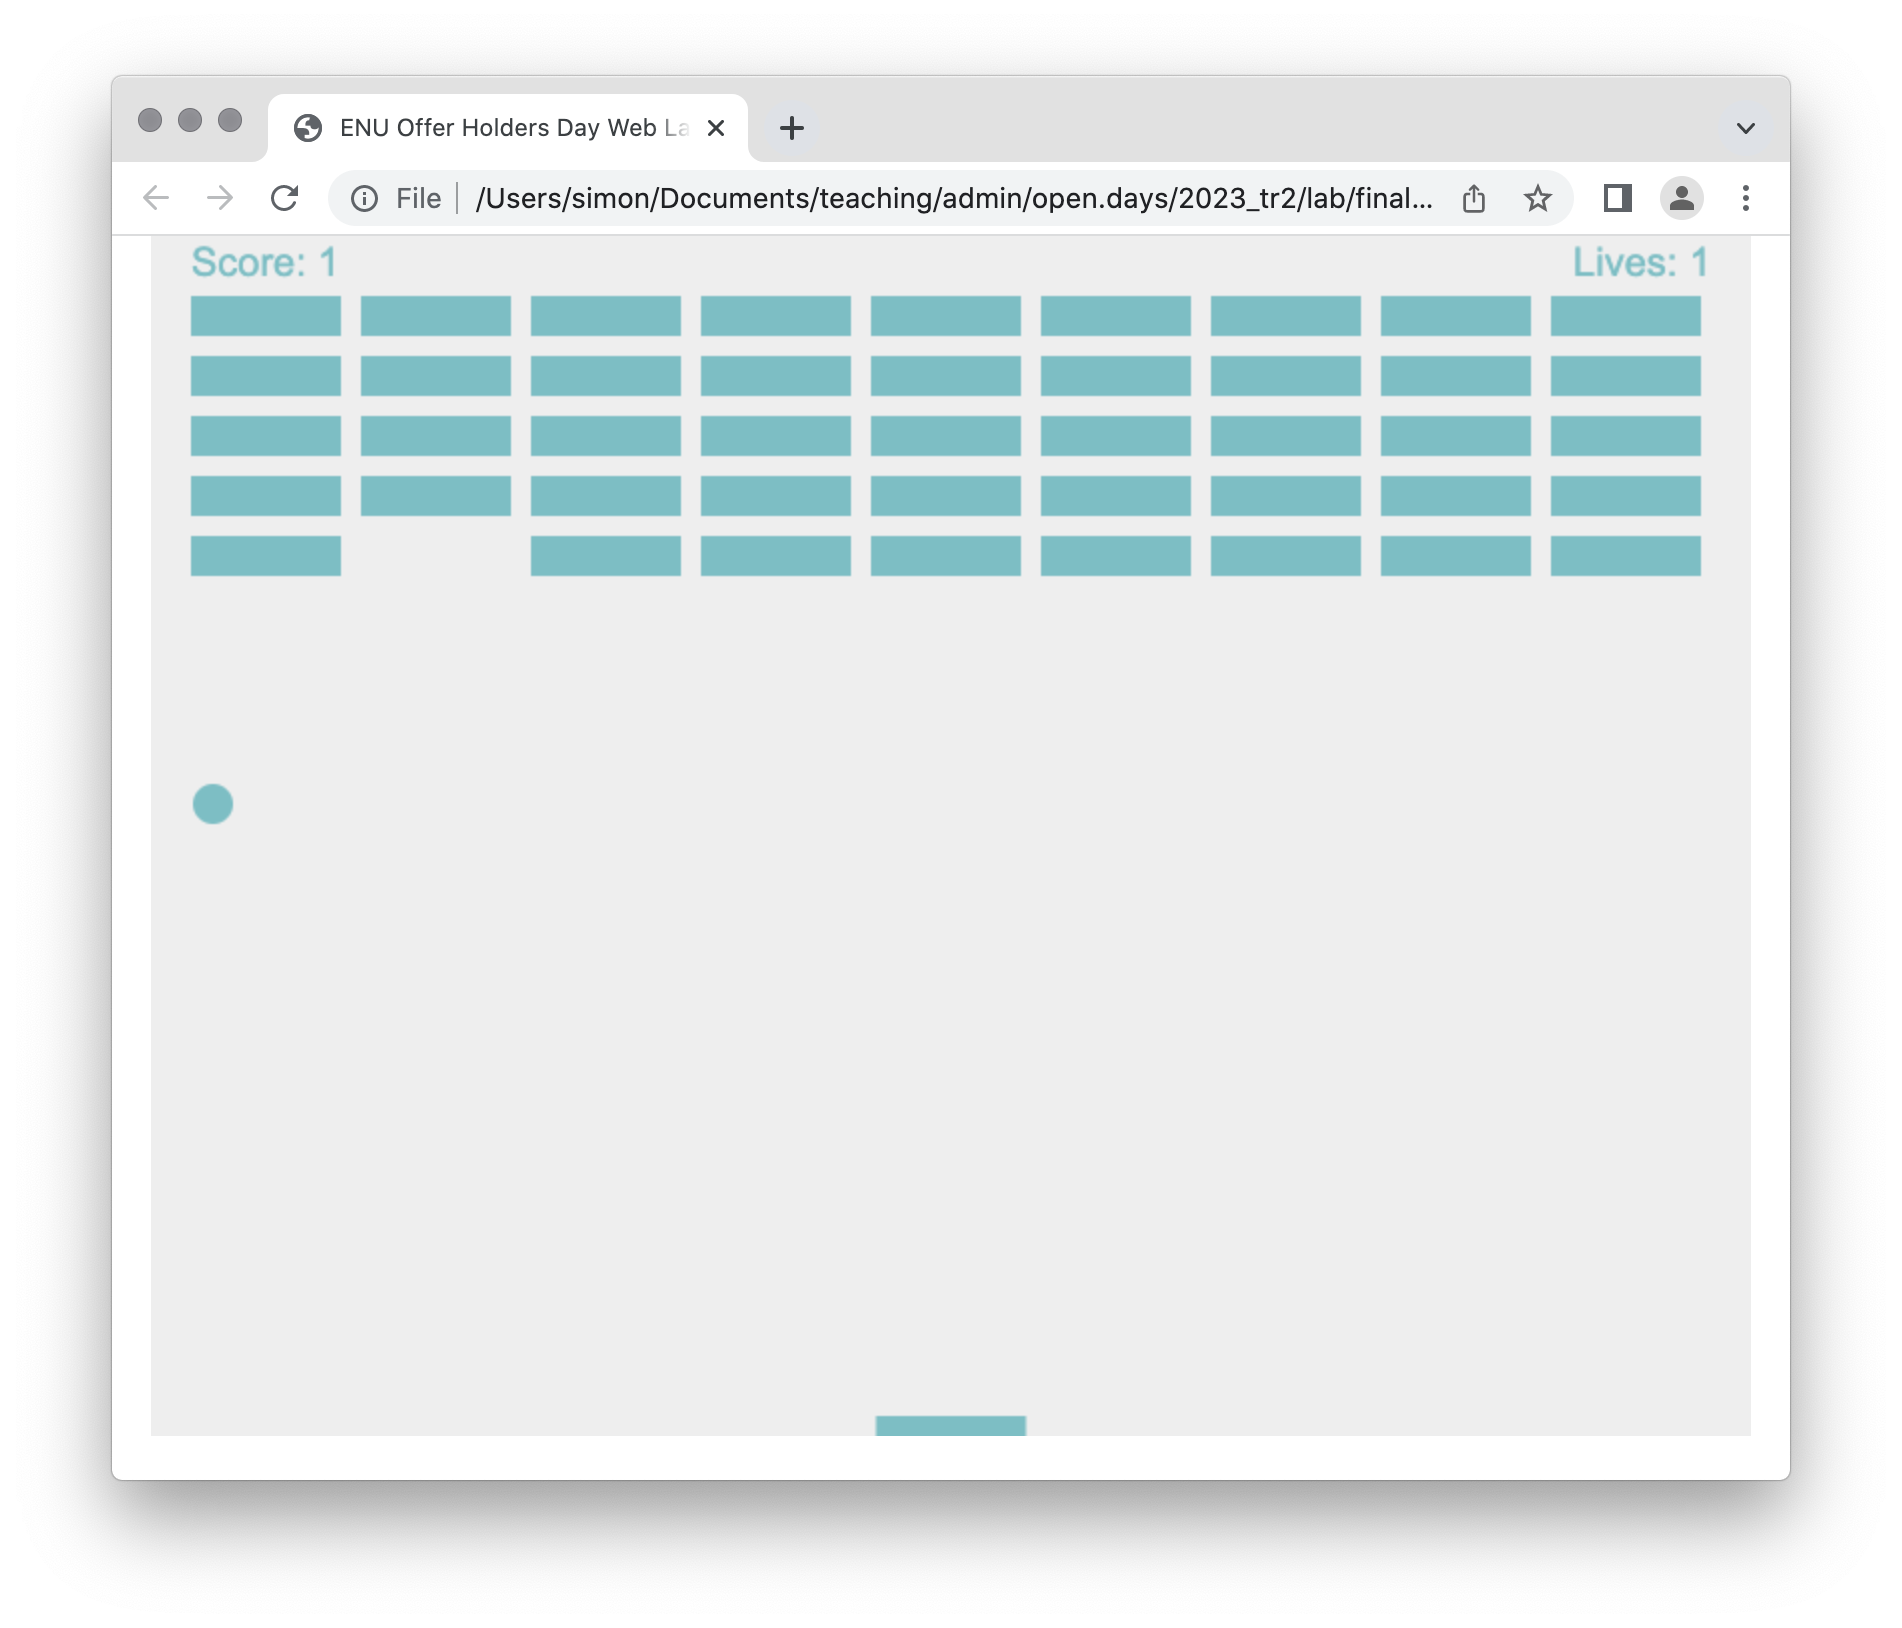
\includegraphics[width=0.8\textwidth]{images/breakout.png}
\caption{The venerable ``breakout'' game.}
\label{fig:breakout}
\end{figure}

\paragraph{} We're going to build this using some HTML, some CSS, and some Javascript, and the resulting game will run entirely within the Chrome web browser. 

\paragraph{} This will look like a lot of work right now, but the game itself is less than 200 lines of code. Most of the sub-activities of this lab involve breaking down that 200 lines into smaller logical sections and then studying what they do in isolation. A lot of the sub-activities also re-show the code over and over as it grows into the final project so much of the bulk of this lab sheet is actually repetition. It is this repetition that bulks out this document, but it helps to see the changes in context as we add new code to code we've written in previous sub-sections. 

\paragraph{} If you want to get the game working first, then feel free to skip to Section \ref{section:collisions}. You might also introduce typos along the way, which strictly speaking means bugs that need to be fixed. To help, the complete source code listing for the game, and each sub-section are available from this Github repository: \url{https://github.com/siwells/offer-holder-day}. Ultimately the aim of this lab is to give you a flavour of the kind of stuff that you can look forward to, as well as giving you a starting place for further exploration. Section \ref{section:challenges} might inspire you with some suggestions for next steps. If you do want to do further explorartion then you'll likely find that digging into what you can do with HTML, CSS, and JS is  good starting place as this lab sheet only scratches the surface.


%\begin{itemize}
%\item 
%\end{itemize}


\paragraph{} 


\section{Activities}

\paragraph{} The following sub-sections each build on each other to construct the complete breakout game.

\subsection{Preliminaries}

\paragraph{} In order to build our game we're going to need three things. 

\begin{itemize}
\item Access to the university system
\item The Chrome Web Browser
\item Notepad
\end{itemize}


\paragraph{} First things first we need to log in to the university system. You should have a username:password combination that you can use to log in today. If you don't have one then please ask one of the members of staff and they'll help you out. When you've logged in you will find a standard Windows desktop.

\paragraph{} We're going to test and run our game within the Chrome Web browser. So launch Chrome in the usual way.

\paragraph{} We're going to need to write some code. Most code is written in an editor before it is executed or otherwise used. There are exceptions to this but for now let's go with it. Our editor for today will be Notepad, Window's built in plain text editor. There are many editors out there and you're encouraged, in the longer term, to find one that you like and which provides the kinds of features that you need in your career as a software developer. However Notepad is simple and available on any version of Windows going back to Windows 1.0 so it's a useful common denominator.

%\begin{lstlisting}

%\end{lstlisting}


\subsection{Skeleton}

\paragraph{} Start notepad and create a new file. Save this file as \emph{game.html} using the ``save as'' option from the save menu. If you don't do this then your file will be saved as a text file instead of as an html file. Now type the following code into your game.html file and save it.

\begin{lstlisting}
<!DOCTYPE html>
<html>
<head>
    <meta charset="utf-8" />
    <title>ENU Offer Holders Day Web Lab</title>
    <style>
        * { 
            padding: 20px; 
            margin: 0; 
        }
    </style>
</head>
<body>
    Any text you put here will turn up on screen... That's how easy it is to create a web page. We can make headings using the h1 tags like so:

    <h1>An example heading</h1>
    <p>and create paragraphs like this using the p tags. Note that headings can range in size from h1 through to h6, getting progressively smaller. This gives you a way to organise the text content of your page into sections.</p>

    <script>

    </script>
</body>
</html>
\end{lstlisting}

\paragraph{} This is just a simple web page. It doesn't yet have any Javascript. We'll add that soon in the section between the opening $<$script$>$ and closing $<$/script$>$ tags in line 20. Notice that you can pick out a closing tag because it contain a forward slash ``/''. As a rule, most HTML tags come in pairs, the opening and closing tag for whichever HTML \emph{keyword} you're dealing with.

\paragraph{} Line 1 tells the browser that this file is an HTML file. Lines 2 and 23 are the opening and closing tags for the HTML document. An HTML document always has two main sections, the head section and the body seciotn. The opening and closing head tags are in lines 3 and 12, and the opening and closing body tags are in lines 13 and 22. Line 4 specifies how the contents of this HTML document are encoded. Line 5 is used to create the document's title, the thing that is displayed in the tab text when the file is opened in a Web browser. Lines 6 and 11 are the opening and closing tags for the style section, which is used to influence how the page is visually depicted. Within the style section, in lines 7 to 10, there is a small bit of CSS which is used to give us a slightly nice user interface once our page is loaded into the browser. In the body section we have some text and some example text-oriented HTML tags, which is just there to give us something to see when we load this into the browser. We'll delete lines 14 to 18 late and replace them with something else. This does show though how straightforward it is to create a web page. The Web was actually designed initially to be something that anyone could publish to with a minimal of programming skills. To a large degree this is actually still the case.

\paragraph{} Open your game.html file in Chrome. You can do this by starting Chrome and using the File $\to$ Open File menu option, or by dragging your game.html file from the windows explorer onto your Chrome Window. You might even be able to double click you game.html file and have it loaded into Chrome. Note that how this works all depends on how your specific machine is set up so just see what works and if you get stuck, seek assistance from a demonstrator, member of staff, or even the person sitting next to you.

\paragraph{} Your page should now look something like this:

\begin{figure}[H]
\centering
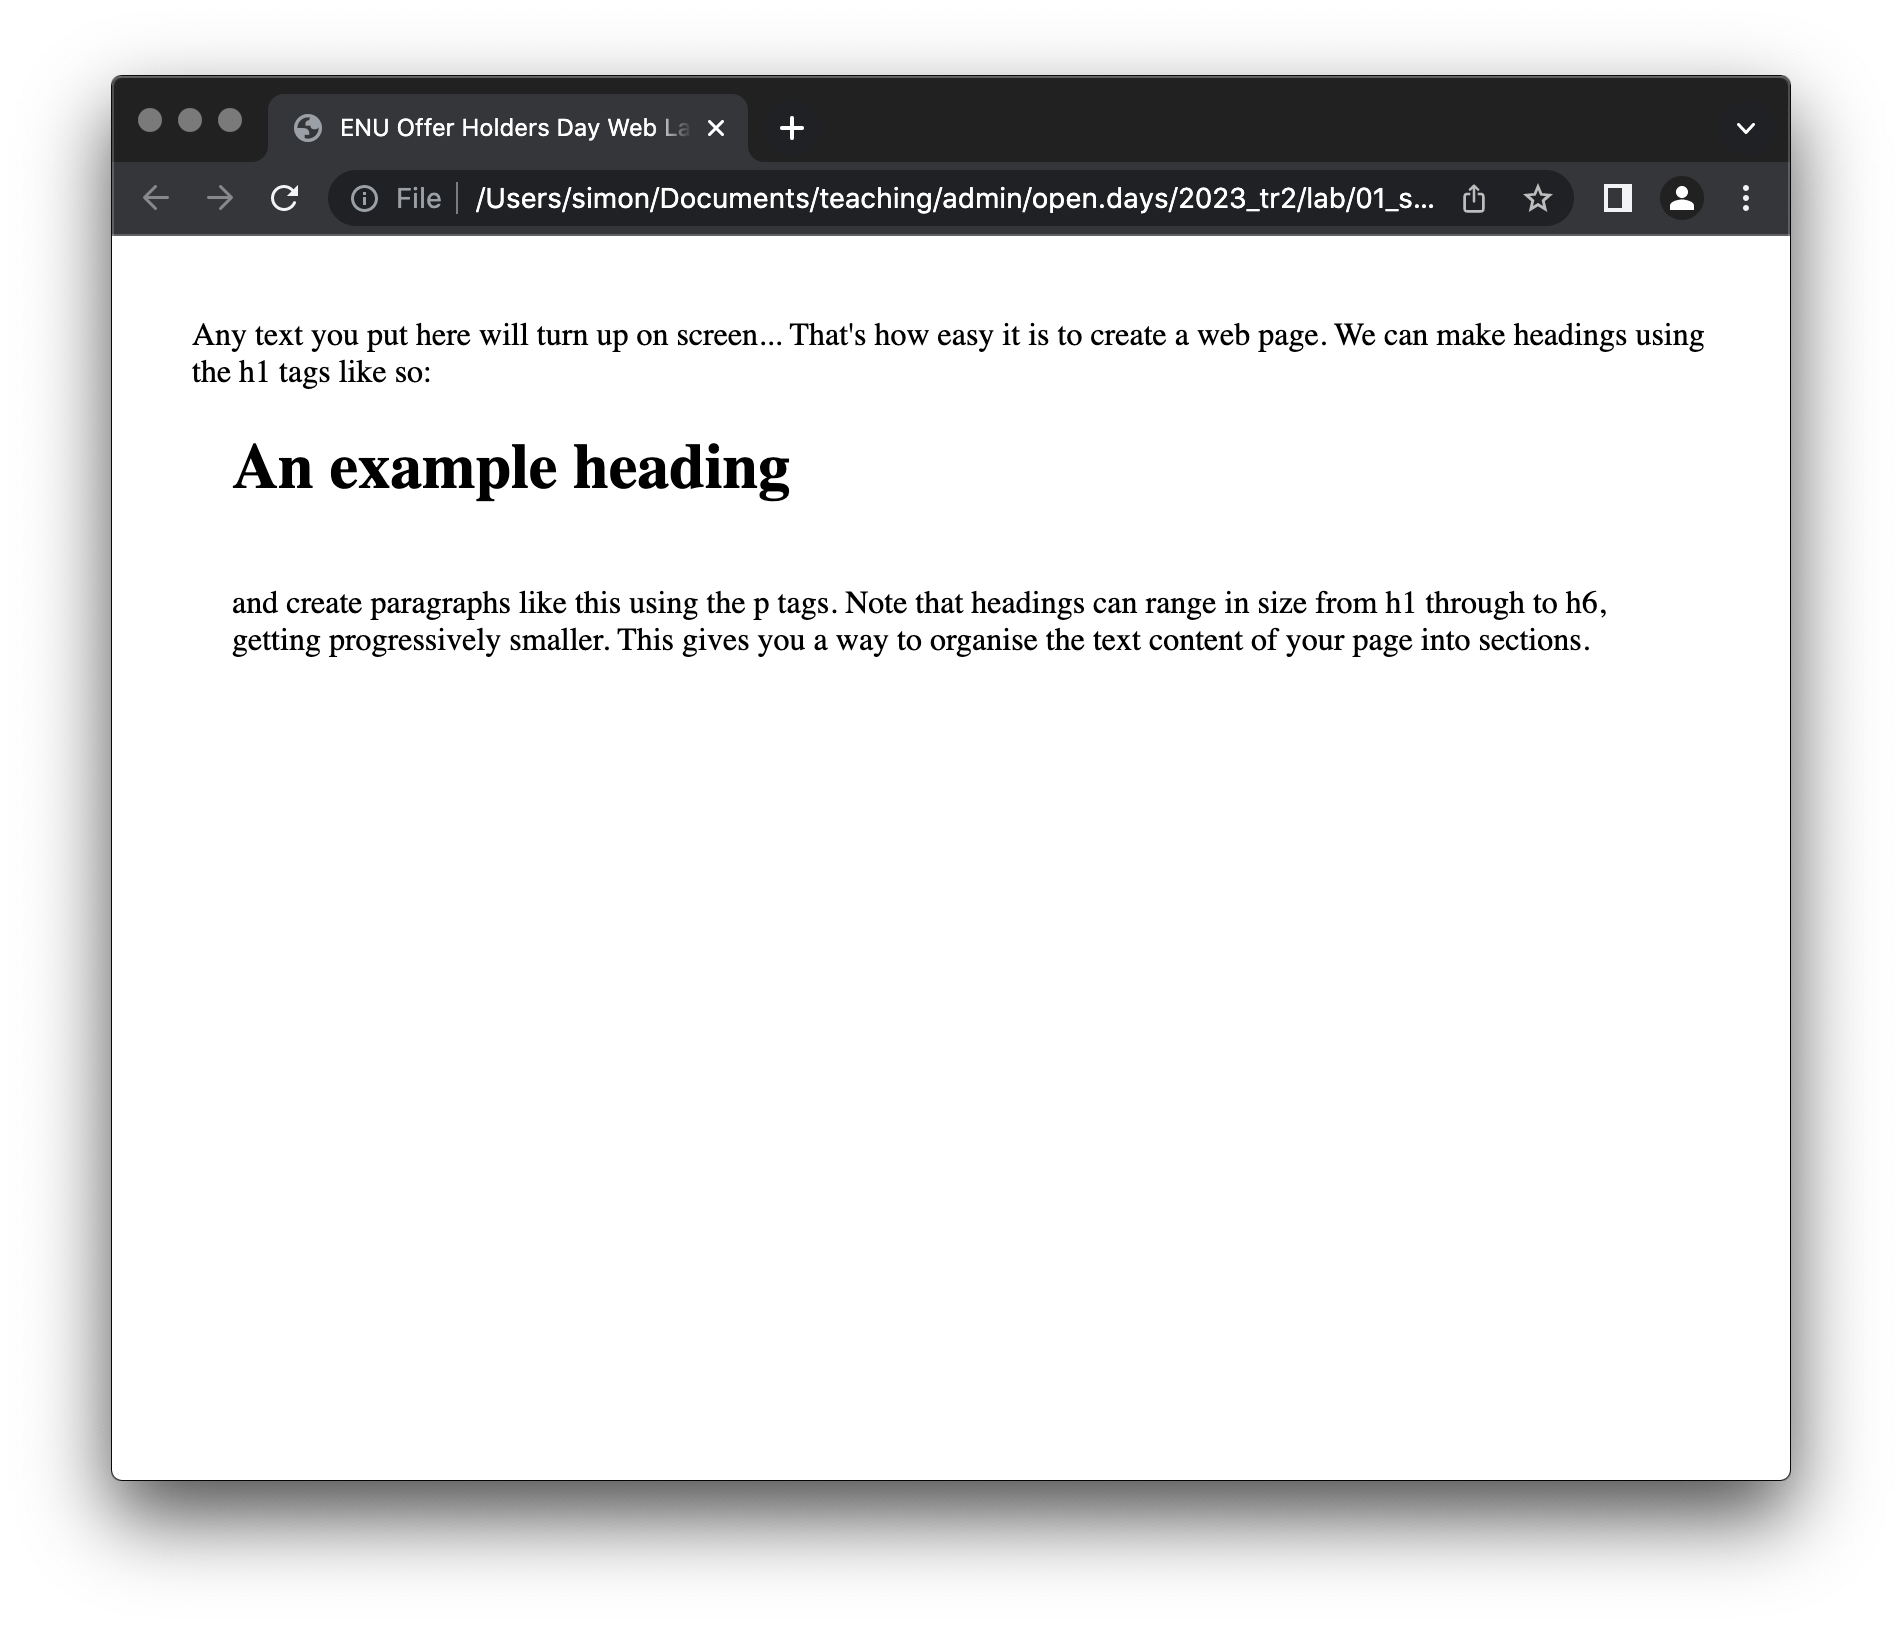
\includegraphics[width=0.8\textwidth]{images/01_skeleton+skeleton.png}
\caption{The basic skeleton for our game.}
\label{fig:01_skeleton+skeleton}
\end{figure}


\subsection{Drawing}

\paragraph{} The part of our game that faces the user, the interface, is the first thing we'll create. Take a look at the screenshot in Figure \ref{fig:breakout} and notice that it is built from four elements:

\begin{itemize}
\item The Ball
\item The Paddle
\item The Blocks
\item The Score \& Lives text
\end{itemize}

\paragraph{} We'll create each, one at a time, as separate \emph{functions}. That is, sections of code that we can execute and reuse as necessary in our game. This is because it turns out that most games, in fact most programmes, are actually built from pieces of code that are grouped together to encapsulate a specific function, and then these are run repeatedly. For example, in our game the ball will need to be redrawn very frequently to reflect it's moving around the screen and colliding with the walls, blocks, and paddle.

\paragraph{} So let's draw the ball. Edit your game.html file as follows:

\begin{lstlisting}
<!DOCTYPE html>
<html>
<head>
    <meta charset="utf-8" />
    <title>ENU Offer Holders Day Web Lab</title>
    <style>
        * { 
            padding: 0; 
            margin: 0; 
        } 
        canvas { 
            padding: 0; 
            margin: auto; 
            background: #eee; 
            display: block; 
        }
   </style>
</head>
<body>
    <canvas id="game_canvas" width="800" height="600"></canvas>

    <script>
        var canvas = document.getElementById("game_canvas");
        var ctx = canvas.getContext("2d");
        var ball_radius = 10;
        var x = canvas.width-Math.floor(Math.random()*750);
        var y = canvas.height-(Math.floor(Math.random()*200)+50);
        var colour = get_random_colour();


        function get_random_colour() {
            return '#'+Math.floor(Math.random()*16777215).toString(16);
        }

        function draw_ball() {
            ctx.beginPath();
            ctx.arc(x, y, ball_radius, 0, Math.PI*2);
            ctx.fillStyle = colour;
            ctx.fill();
            ctx.closePath();
        }
        draw_ball();
    </script>
</body>
</html>

\end{lstlisting}

\paragraph{} Much of the code is the same as before except that we've deleted the original text between the $<$body$>$ and $<$script$>$ tags then made some additions. The additions are as follows:

\begin{description}
\item[Line 20] We created an HTML canvas element. A canvas is a place for drawing. We've basically allocated an area of the web page, 600 pixels high and 800 pixels wide, in which we will draw the elements of our breakout game.
\item[Line 23] We created a JS variable to enable us to interact programmatically with the canvas drawing area on the webpage.
\item[Line 24] We indicate to the browser that we want to draw in 2 dimensions (``2d'') instead of 3D. Perhaps bear this in mind in case you someday want to build a 3D breakout game in the future?
\item[Line 25] A variable for the radius of our ball
\item[Line 26] A variable for the x coordinate of the location of our ball
\item[Line 27] A variable for the y coordinate of the location of our ball
\item[Line 28] A variable holding the colour value in which to draw the game. This actually calls a function that we've created in lines 31--33
\end{description}

\paragraph{} We could have used fixed values for the x and y coodinates in lines 26 \& 27 but that means that the game always starts with the ball in the same place. Instead we've used a maths function to return a bounded random value so that the starting location ofthe ball always lies somewhere between the paddle and the blocks.

\paragraph{} We've also go two functions, one function to set a random colour, which will change everyt time the page is refreshed, and one function to draw the ball.

\begin{description}
\item[Lines 31--33] The get\_random\_colour() function. This just returns a hexadecimal number to the place that called it. The number itself is randomly generated from the space of hexadecimal encoded colours so that we can get a different valid colour code whenever we want.
\item[Lines 35--41] The draw\_ball() function includes some code to draw a ball onto the canvas, using the x \& y coordinates we created earlier. The balls size is set by the radius we set in line 25, and the colour is the one that was created by our call to get\_random\_colour() in line 28. It's useful to think of drawing in JS as being like drawing with a pencil, we apply the pencil in a particular place to make a mark, and then raise it to stop making a mark. If we apply the pencil and move it then we get a line. A lot of drawing in code can be broken down into a sequence of applying the ``pencil'', making a mark, and then raising the ``pencil'' when we're done.
\item[Line 42] Finally, having created our draw\_ball() function, we need to ``call'' it to get the code to run.
\end{description}

\paragraph{} Your page should now look something like this:

\begin{figure}[H]
\centering
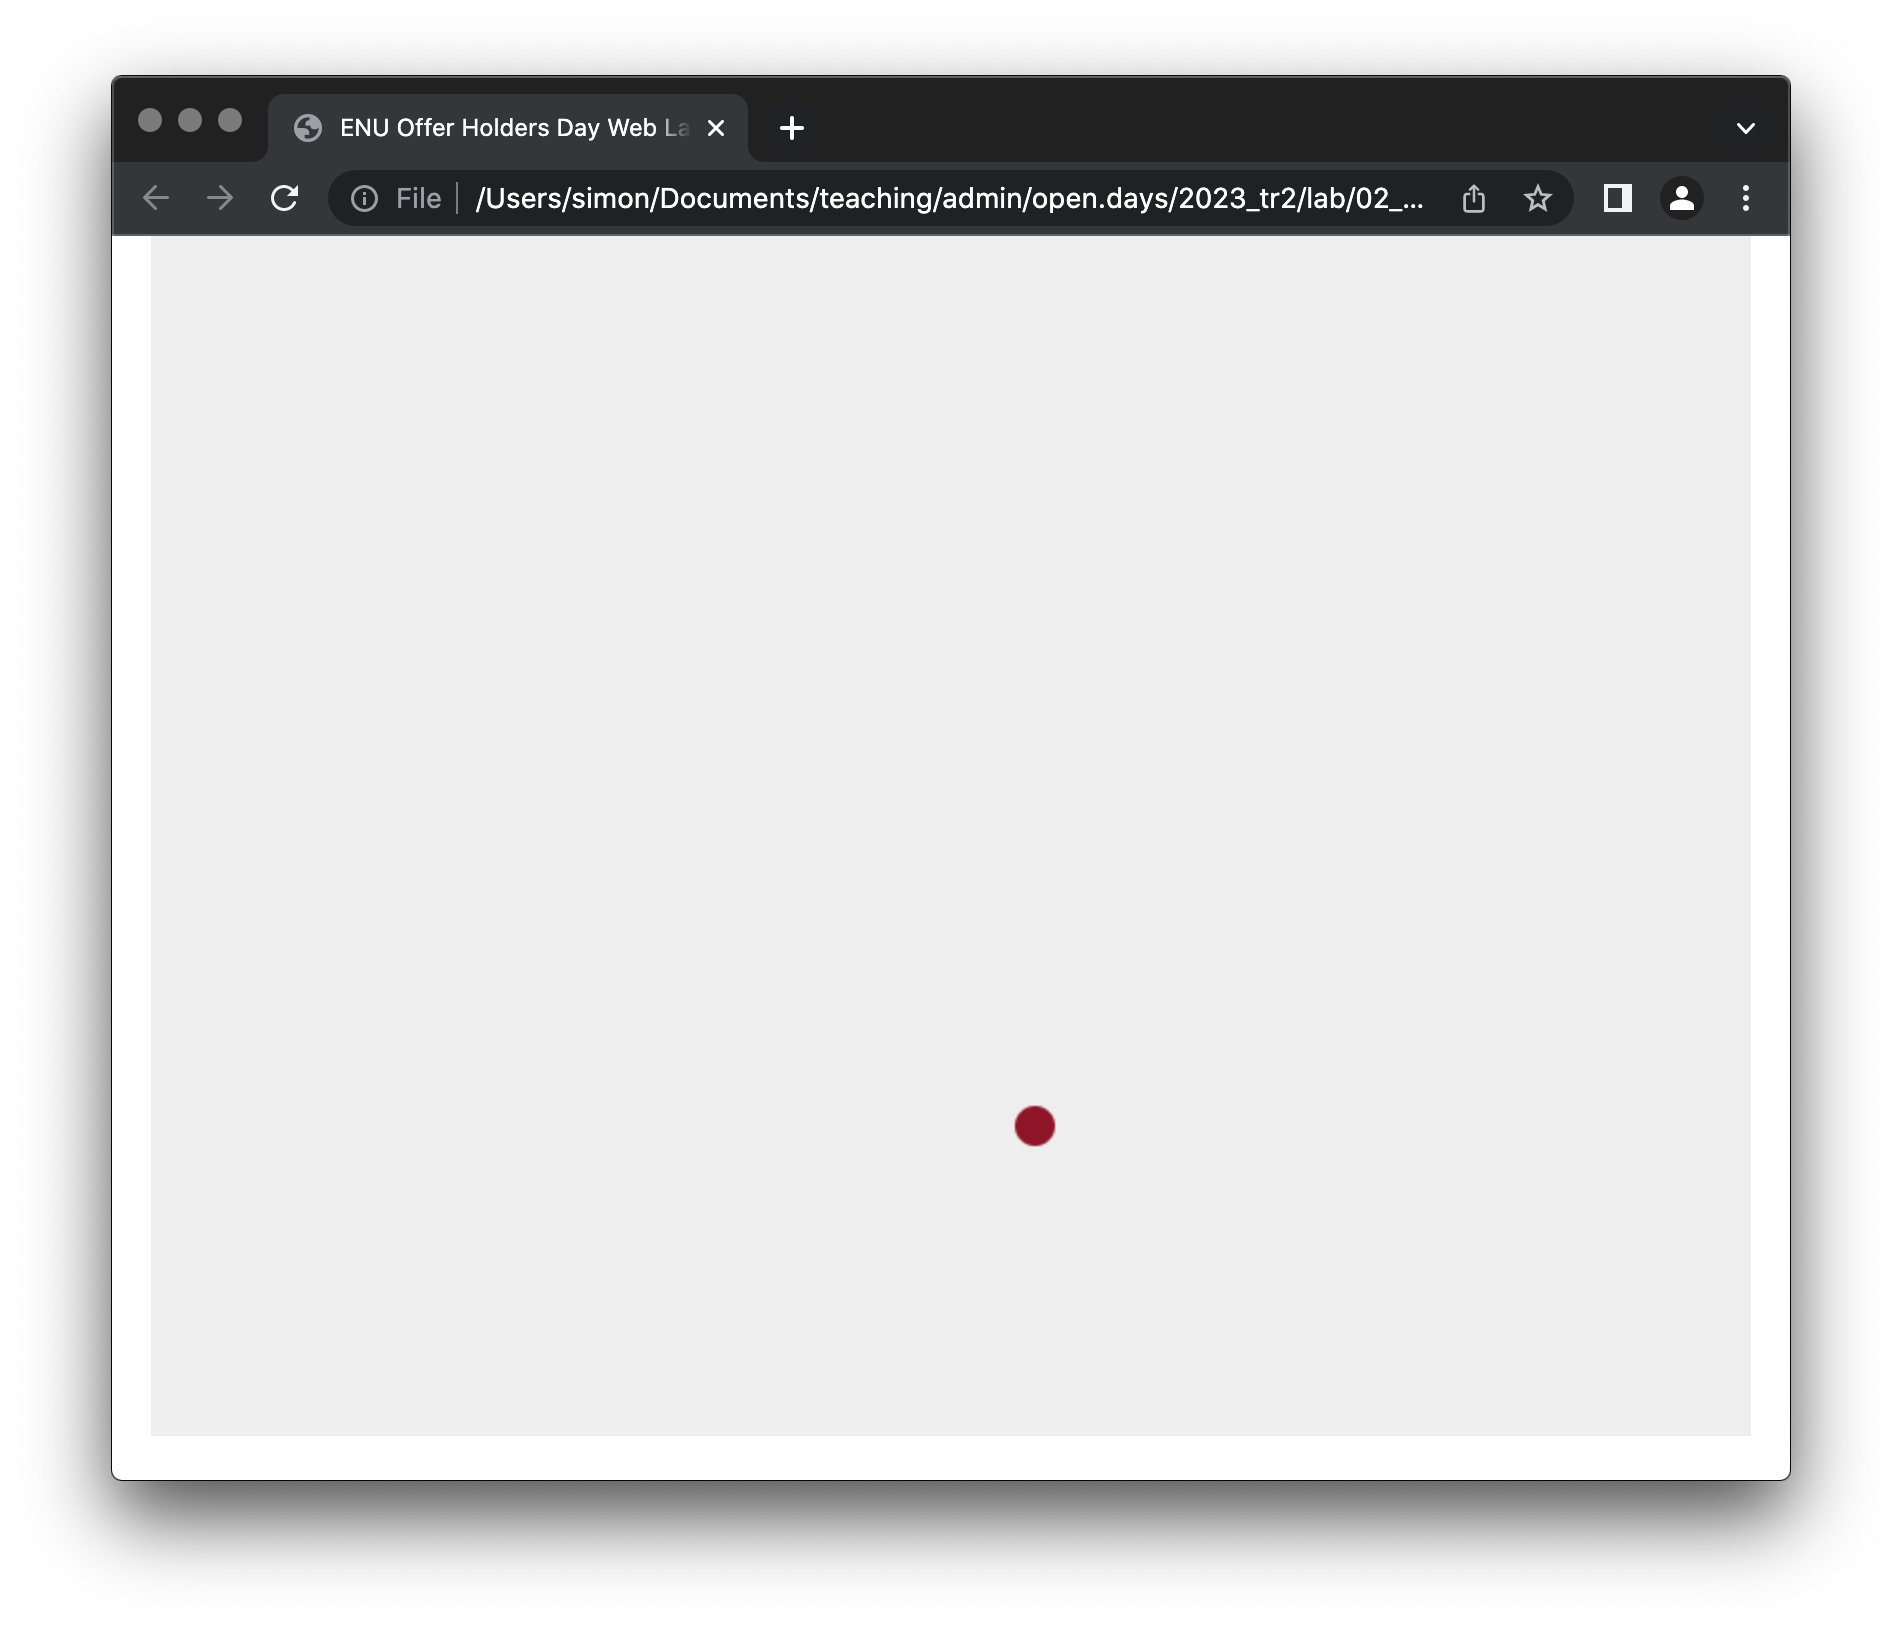
\includegraphics[width=0.8\textwidth]{images/02_drawing+a_draw_ball.png}
\caption{Drawing the ball.}
\label{fig:02_drawing+a_draw_ball}
\end{figure}



\paragraph{} Now we'll draw the paddle. This is just a rectangle that will appear towards the bottom of our campus. The full code listing is as follows which now also contains some code to draw the paddle.

\begin{lstlisting}
<!DOCTYPE html>
<html>
<head>
    <meta charset="utf-8" />
    <title>ENU Offer Holders Day Web Lab</title>
    <style>
        * { 
            padding: 0; 
            margin: 0; 
        } 
        canvas { 
            padding: 0; 
            margin: auto; 
            background: #eee; 
            display: block; 
        }
   </style>
</head>
<body>
    <canvas id="game_canvas" width="800" height="600"></canvas>

    <script>
        var canvas = document.getElementById("game_canvas");
        var ctx = canvas.getContext("2d");
        var ball_radius = 10;
        var x = canvas.width-Math.floor(Math.random()*750);
        var y = canvas.height-(Math.floor(Math.random()*200)+50);
        var paddle_height = 10;
        var paddle_width = 75;
        var paddle_position = (canvas.width-paddle_width)/2;

        var colour = get_random_colour();


        function get_random_colour() {
            return '#'+Math.floor(Math.random()*16777215).toString(16);
        }

         function draw_ball() {
            ctx.beginPath();
            ctx.arc(x, y, ball_radius, 0, Math.PI*2);
            ctx.fillStyle = colour;
            ctx.fill();
            ctx.closePath();
        }

        function draw_paddle() {
            ctx.beginPath();
            ctx.rect(paddle_position, canvas.height-paddle_height, paddle_width, paddle_height);
            ctx.fillStyle = colour;
            ctx.fill();
            ctx.closePath();
        }

 
        draw_ball();
        draw_paddle();
    </script>
</body>
</html>
\end{lstlisting}

\paragraph{} The main changes this time are some variables to store some parameters for our paddle, a function to draw the paddle, and a call to execute the paddle drawing function.

\begin{description}
\item[Lines 28--30] Create variables to store the height and width of the paddle along with the initial location in which to draw it.
\item[Lines 47--53] Here we create the draw\_paddle() function which will cause the paddle to be drawn onto the canvas when it is called. Compare the code in this function to what we have in the draw\_ball() function. Both draw a path (remember that pencil metaphor from earlier). However instead of drawing an arc, this time we're drawing a rectangle by specifing four things, the x coordinate of the upper-left corner of the rectangle, the y-coorindate of the upper-left corner of the rectangle, the width of the rectangle, the height of the rectangle in pixels and the width of the rectangle in pixels.
\item[Line 57] And finally, we draw the paddle by calling the draw\_paddle() function.
\end{description}

\paragraph{} Open the breakout.html file in Chrome and see how it looks. Your page should now look something like this:

\begin{figure}[H]
\centering
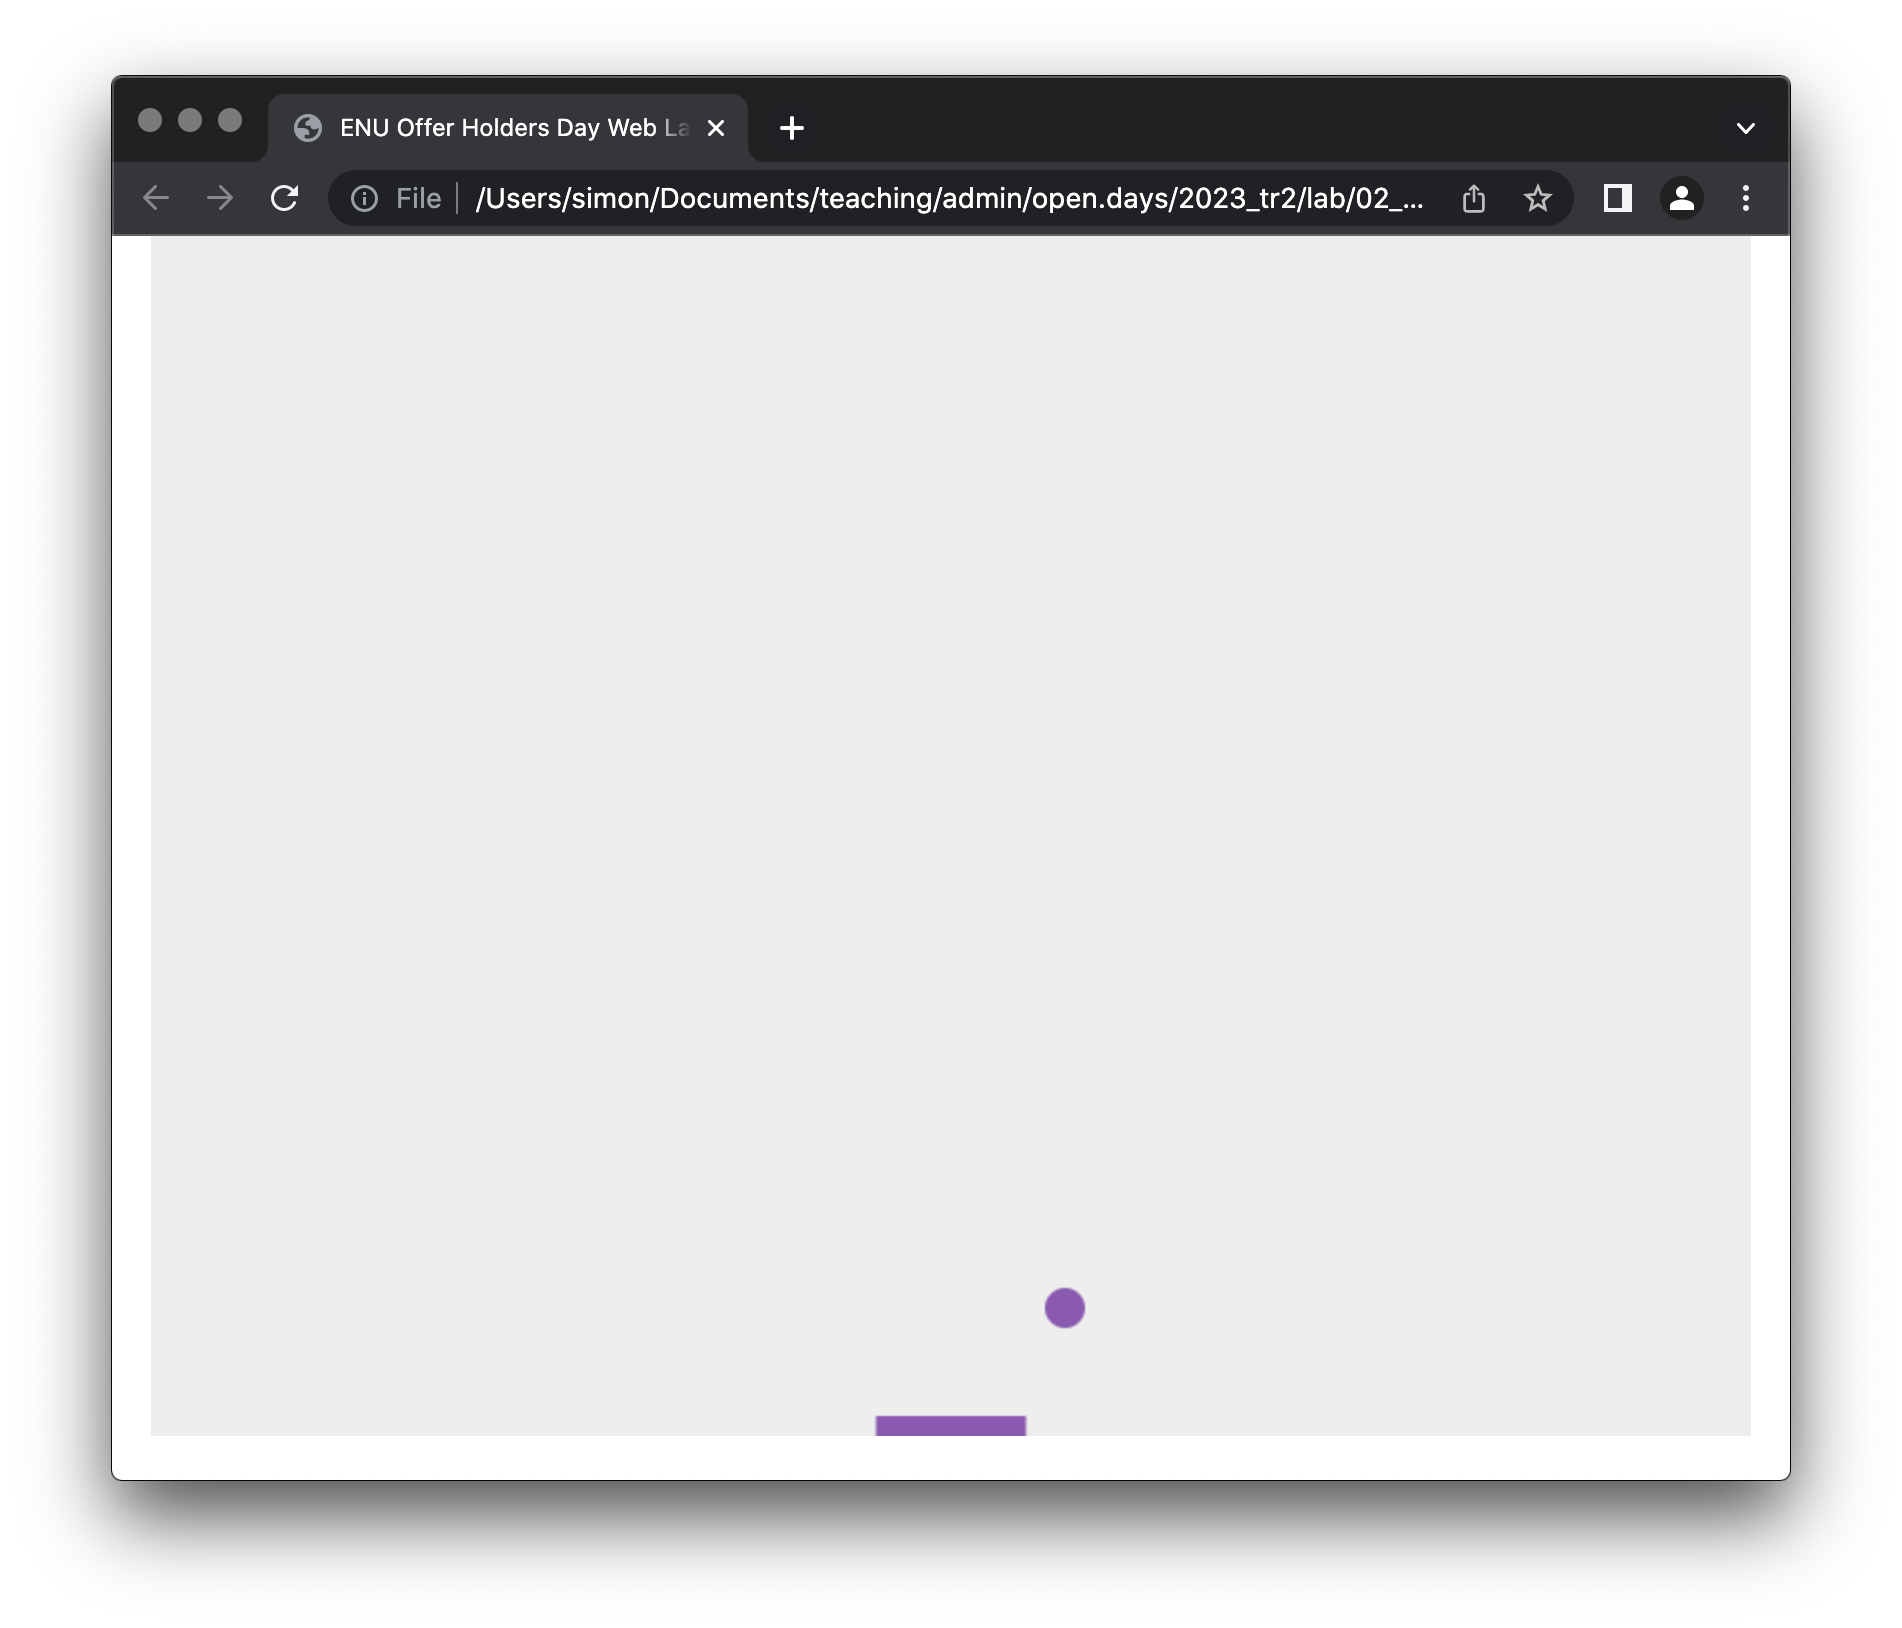
\includegraphics[width=0.8\textwidth]{images/02_drawing+b_draw_paddle.png}
\caption{Drawing the paddle.}
\label{fig:02_drawing+b_draw_paddle}
\end{figure}


\paragraph{} Hopefuly you should be noticing some patterns now in how we're building things. Having created the initial skeleton we're basically adding new variables and new functions, and then calling them.

\paragraph{} Now let's draw the blocks:

\begin{lstlisting}
<!DOCTYPE html>
<html>
<head>
    <meta charset="utf-8" />
    <title>ENU Offer Holders Day Web Lab</title>
    <style>
        * { 
            padding: 0; 
            margin: 0; 
        } 
        canvas { 
            padding: 0; 
            margin: auto; 
            background: #eee; 
            display: block; 
        }
   </style>
</head>
<body>
    <canvas id="game_canvas" width="800" height="600"></canvas>

    <script>
        var canvas = document.getElementById("game_canvas");
        var ctx = canvas.getContext("2d");
        var ball_radius = 10;
        var x = canvas.width-Math.floor(Math.random()*750);
        var y = canvas.height-(Math.floor(Math.random()*200)+50);
        var paddle_height = 10;
        var paddle_width = 75;
        var paddle_position = (canvas.width-paddle_width)/2;
        var block_column_count = 9;
        var block_row_count = 5;
        var block_height = 20;
        var block_width = 75;
        var gutter = 10;
        var padding = 30;
        var top_margin = 20;
        var inside_margin = 20;

        var blocks = [];
        var colour = get_random_colour();

        function get_random_colour() {
            return '#'+Math.floor(Math.random()*16777215).toString(16);
        }

        function build_wall() {
            for(var c=0; c<block_row_count; c++) {
                blocks[c] = [];
                for(var r=0; r<block_column_count; r++) {
                    blocks[c][r] = { x: 0, y: 0, status: 1 };
                }
            }
        }
        build_wall();
  
        function draw_ball() {
            ctx.beginPath();
            ctx.arc(x, y, ball_radius, 0, Math.PI*2);
            ctx.fillStyle = colour;
            ctx.fill();
            ctx.closePath();
        }

        function draw_paddle() {
            ctx.beginPath();
            ctx.rect(paddle_position, canvas.height-paddle_height, paddle_width, paddle_height);
            ctx.fillStyle = colour;
            ctx.fill();
            ctx.closePath();
        }

        function draw_blocks() {
            for(var c=0; c<block_row_count; c++) {
                for(var r=0; r<block_column_count; r++) {
                    if(blocks[c][r].status == 1) {
                        var blockX = (r*(block_width+gutter))+inside_margin;
                        var blockY = (c*(block_height+gutter))+padding;
                        blocks[c][r].x = blockX;
                        blocks[c][r].y = blockY;
                        ctx.beginPath();
                        ctx.rect(blockX, blockY, block_width, block_height);
                        ctx.fillStyle = colour;
                        ctx.fill();
                        ctx.closePath();
                    }
                }
            }
        }

        draw_blocks();
        draw_ball();
        draw_paddle();
    </script>
</body>
</html>
\end{lstlisting}

\paragraph{} We've followed a similar pattern this time, but in addition to our draw function, draw\_blocks(), we've got an additional build\_wall() function. This is mainly because the wall is a little more complex than just drawing a single block, as we did for the paddle. Also, when we play a game later, we want to track which blocks have been destroyed by the ball and which haven't. So we're going to create a place to store information about our blocks, then we're going to initialise the values for the blocks, then we're going to drawn them.

\begin{description}
\item[Lines 31--40] Here we create a number of variables to govern the dimensions of our blocks (blocl\_height and block\_width), how many blocks to create (block\_row\_count and block\_column\_count). the horizontal and vertical spacing between the blocks (gutter and padding), and the space between the wall and the borders of our canvas (top\_margin and inside\_margin). We also create a variable in line 40 that stores an array of blocks. This basically means that we want to store infomation about the entire collection of blocks that make up our wall.
\item[Lines 47--54] This is our function to initalise the blocks array with new blocks. For each block we store it's location as a pair of x and y coordinates, and the status of the block.
\item[Line 55] Having created our build\_wall() function we now need to call it. We'll only need to do this once at the beginning of the game. As our game progresses the status of the various blocks will be altered to reflect that they've been hit and destroyed by the ball.
\item[Lines 73--89] Our drawing function for the wall, draw\_blocks(). This is very similar to our previous draw\_paddle function but this time we need to draw many rectangles so we have to loop through the blocks array, drawing each block into it's location. Note that there is also a check on line 76 to determine the status of the block so that destroyed blocks aren't drawn as the game progresses.
\end{description}

\paragraph{} Open the breakout.html file in Chrome and see how it looks. Your page should now look something like this:

\begin{figure}[H]
\centering
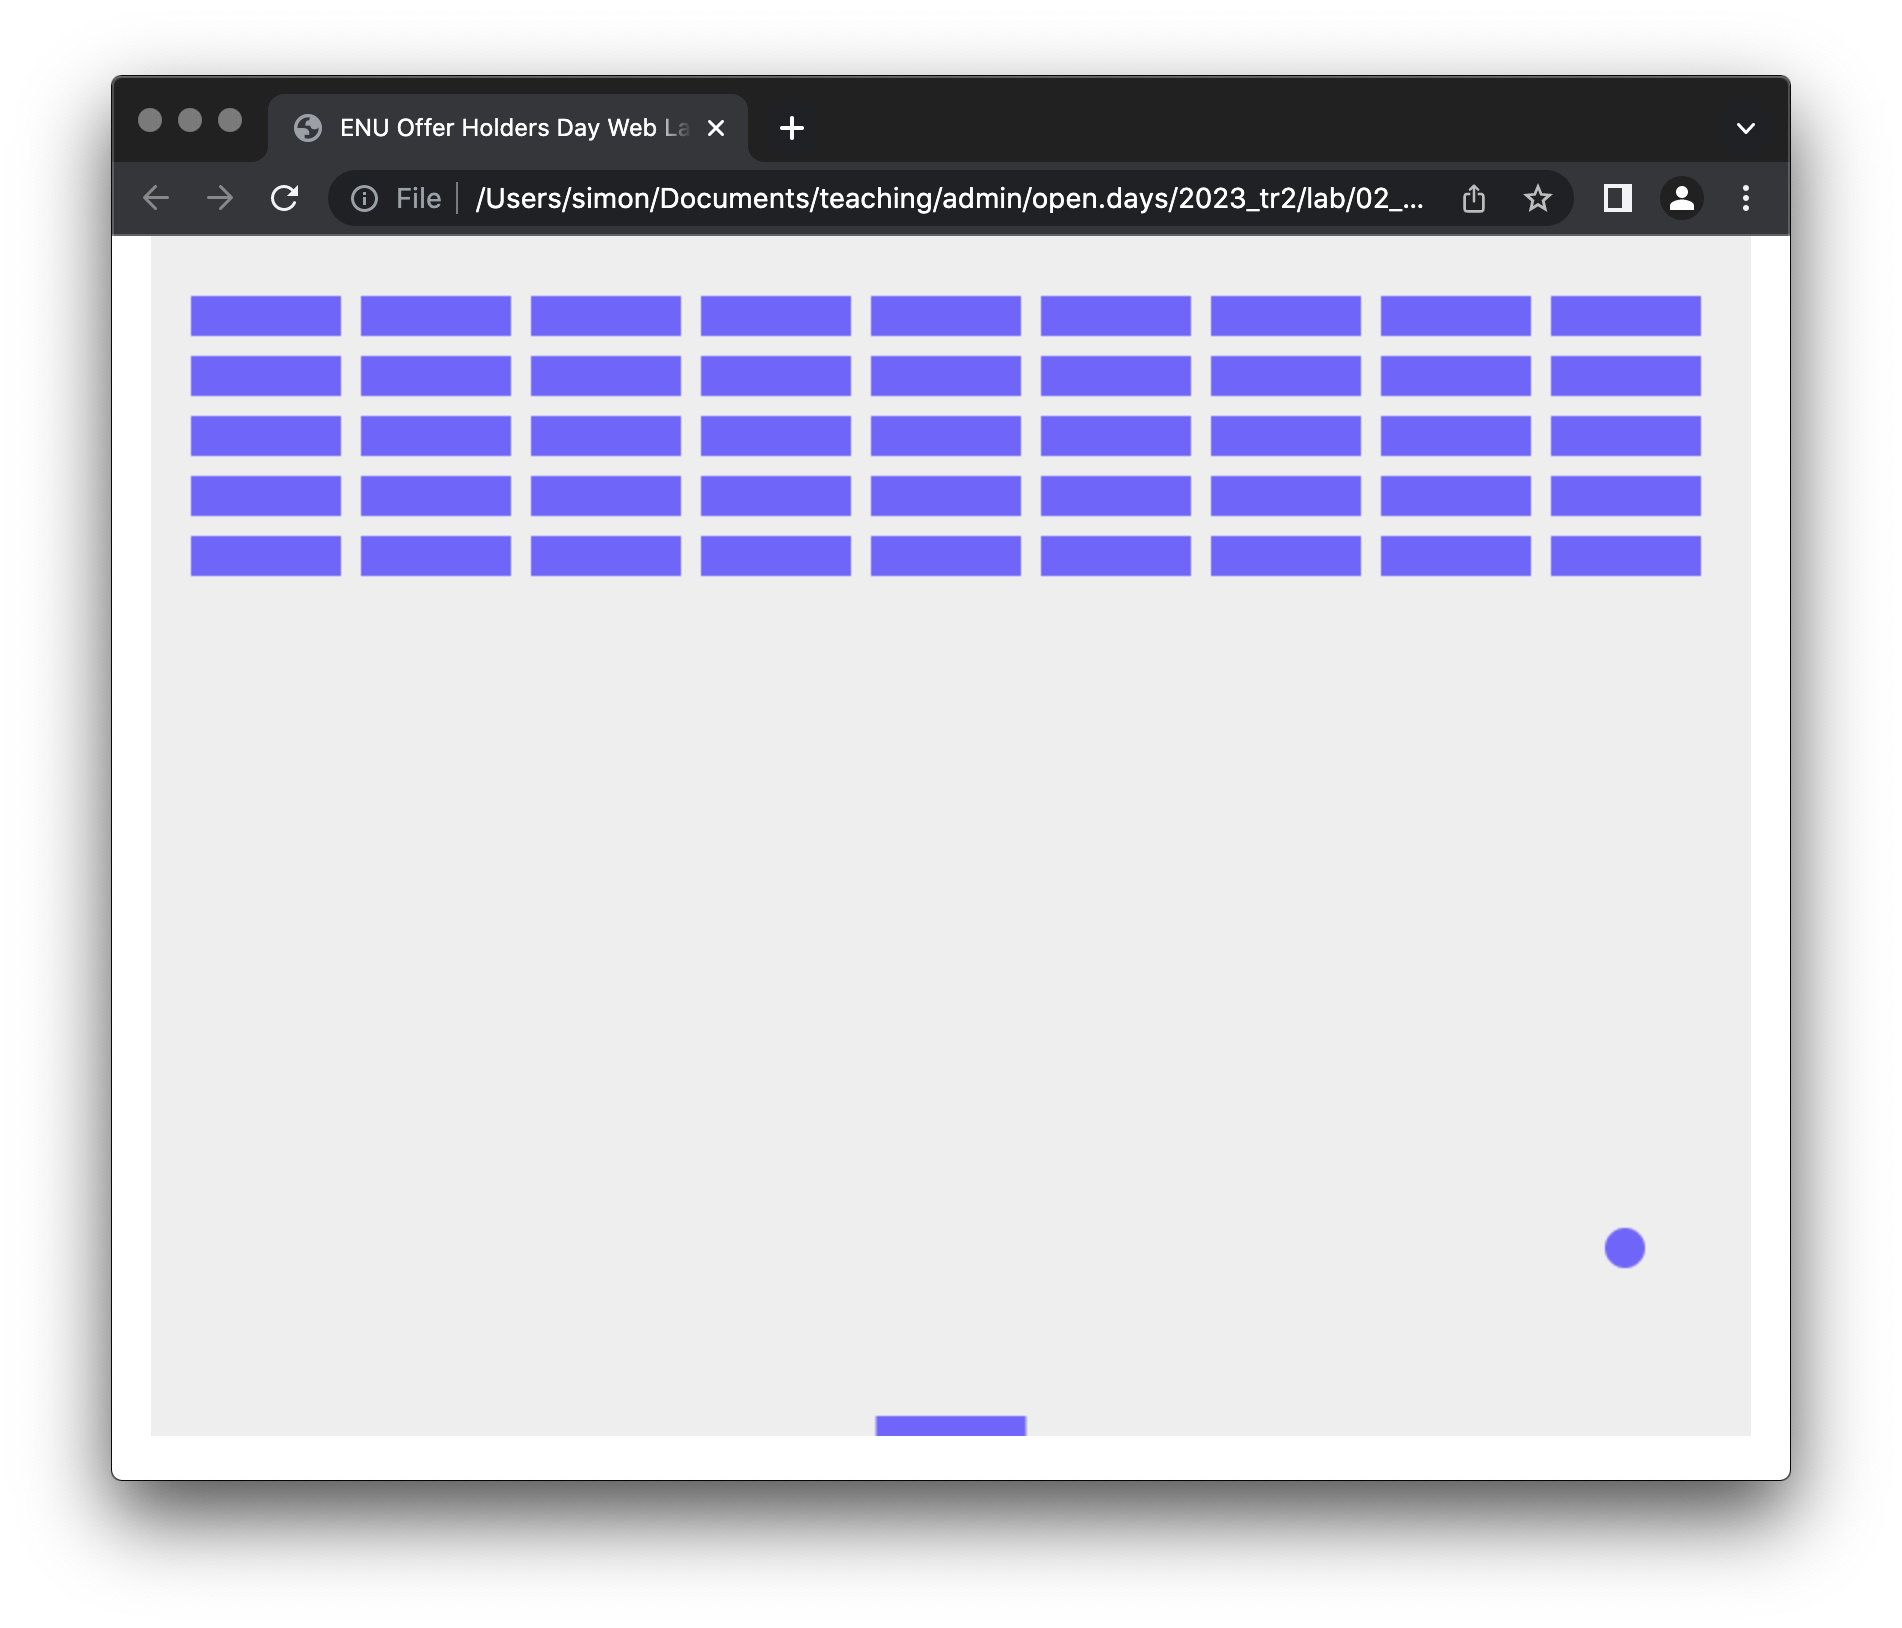
\includegraphics[width=0.8\textwidth]{images/02_drawing+c_draw_blocks.png}
\caption{Drawing the blocks.}
\label{fig:02_drawing+c_draw_blocks}
\end{figure}


\paragraph{} Finally, let's draw the text for the score and number of lives.

\begin{lstlisting}
<!DOCTYPE html>
<html>
<head>
    <meta charset="utf-8" />
    <title>ENU Offer Holders Day Web Lab</title>
    <style>
        * { 
            padding: 0; 
            margin: 0; 
        } 
        canvas { 
            padding: 0; 
            margin: auto; 
            background: #eee; 
            display: block; 
        }
   </style>
</head>
<body>
    <canvas id="game_canvas" width="800" height="600"></canvas>

    <script>
        var canvas = document.getElementById("game_canvas");
        var ctx = canvas.getContext("2d");
        var ball_radius = 10;
        var x = canvas.width-Math.floor(Math.random()*750);
        var y = canvas.height-(Math.floor(Math.random()*200)+50);
        var paddle_height = 10;
        var paddle_width = 75;
        var paddle_position = (canvas.width-paddle_width)/2;
        var block_column_count = 9;
        var block_row_count = 5;
        var block_height = 20;
        var block_width = 75;
        var gutter = 10;
        var padding = 30;
        var top_margin = 20;
        var inside_margin = 20;

        var score = 0;
        var lives = 1;
        var blocks = [];
        var colour = get_random_colour();

        function get_random_colour() {
            return '#'+Math.floor(Math.random()*16777215).toString(16);
        }

        function build_wall() {
            for(var c=0; c<block_row_count; c++) {
                blocks[c] = [];
                for(var r=0; r<block_column_count; r++) {
                    blocks[c][r] = { x: 0, y: 0, status: 1 };
                }
            }
        }
        build_wall();

        function draw_ball() {
            ctx.beginPath();
            ctx.arc(x, y, ball_radius, 0, Math.PI*2);
            ctx.fillStyle = colour;
            ctx.fill();
            ctx.closePath();
        }

        function draw_paddle() {
            ctx.beginPath();
            ctx.rect(paddle_position, canvas.height-paddle_height, paddle_width, paddle_height);
            ctx.fillStyle = colour;
            ctx.fill();
            ctx.closePath();
        }

        function draw_blocks() {
            for(var c=0; c<block_row_count; c++) {
                for(var r=0; r<block_column_count; r++) {
                    if(blocks[c][r].status == 1) {
                        var blockX = (r*(block_width+gutter))+inside_margin;
                        var blockY = (c*(block_height+gutter))+padding;
                        blocks[c][r].x = blockX;
                        blocks[c][r].y = blockY;
                        ctx.beginPath();
                        ctx.rect(blockX, blockY, block_width, block_height);
                        ctx.fillStyle = colour;
                        ctx.fill();
                        ctx.closePath();
                    }
                }
            }
        }

        function draw_score_text() {
            ctx.font = "20px Arial";
            ctx.fillStyle = colour;
            txt  = "Score: "+score;
            ctx.fillText(txt, inside_margin, top_margin);
        }

        function draw_lives_text() {
            ctx.font = "20px Arial";
            ctx.fillStyle = colour;
            txt = "Lives: "+lives;
            ctx.fillText(txt, canvas.width-(ctx.measureText(txt).width + inside_margin), top_margin );
        }
       
        draw_blocks();
        draw_ball();
        draw_paddle();
        draw_score_text();
        draw_lives_text();
    </script>
</body>
</html>
\end{lstlisting}

\paragraph{} Similar to before, a couple of variables, a couple of functions, and a call to execute those functions.

\begin{description}
\item[Lines 40--41] Two variables to hold the players current score and the number of remaining lives.
\item[Lines 93--98] A function to draw the text for the score, draw\_score\_text(). Note that this uses a different canvas drawing function, the filltext() function to draw text into our canvas in a specified location.
\item[Lines 100--105] Similar to the last function this one draw\_lives\_text() is used to display the number of lives our player has. Becuase this text is right-aligned there is a slightly more complex calculation to determing where to start drawing the text as we have to calculate how big the text will be, using he measureText() function, and then adjust the starting place for drawing the text into the canvas as a result.
\item[Lines 110-111] Actually call our functions to draw the score and number of lives.
\end{description}

\paragraph{} And that's it. All the code we need for drawing the user interface for our game. The rest of the code is about getting these drawing functions to act like a game by moving things around, checking for collisions, and checking whether the game is finished. However we don't really have a game yet. All we have is something that draws how the game looks but we can't interact with it, and nothing moves.

\paragraph{} Open the breakout.html file in Chrome and see how it looks. Your page should now look something like this:

\begin{figure}[H]
\centering
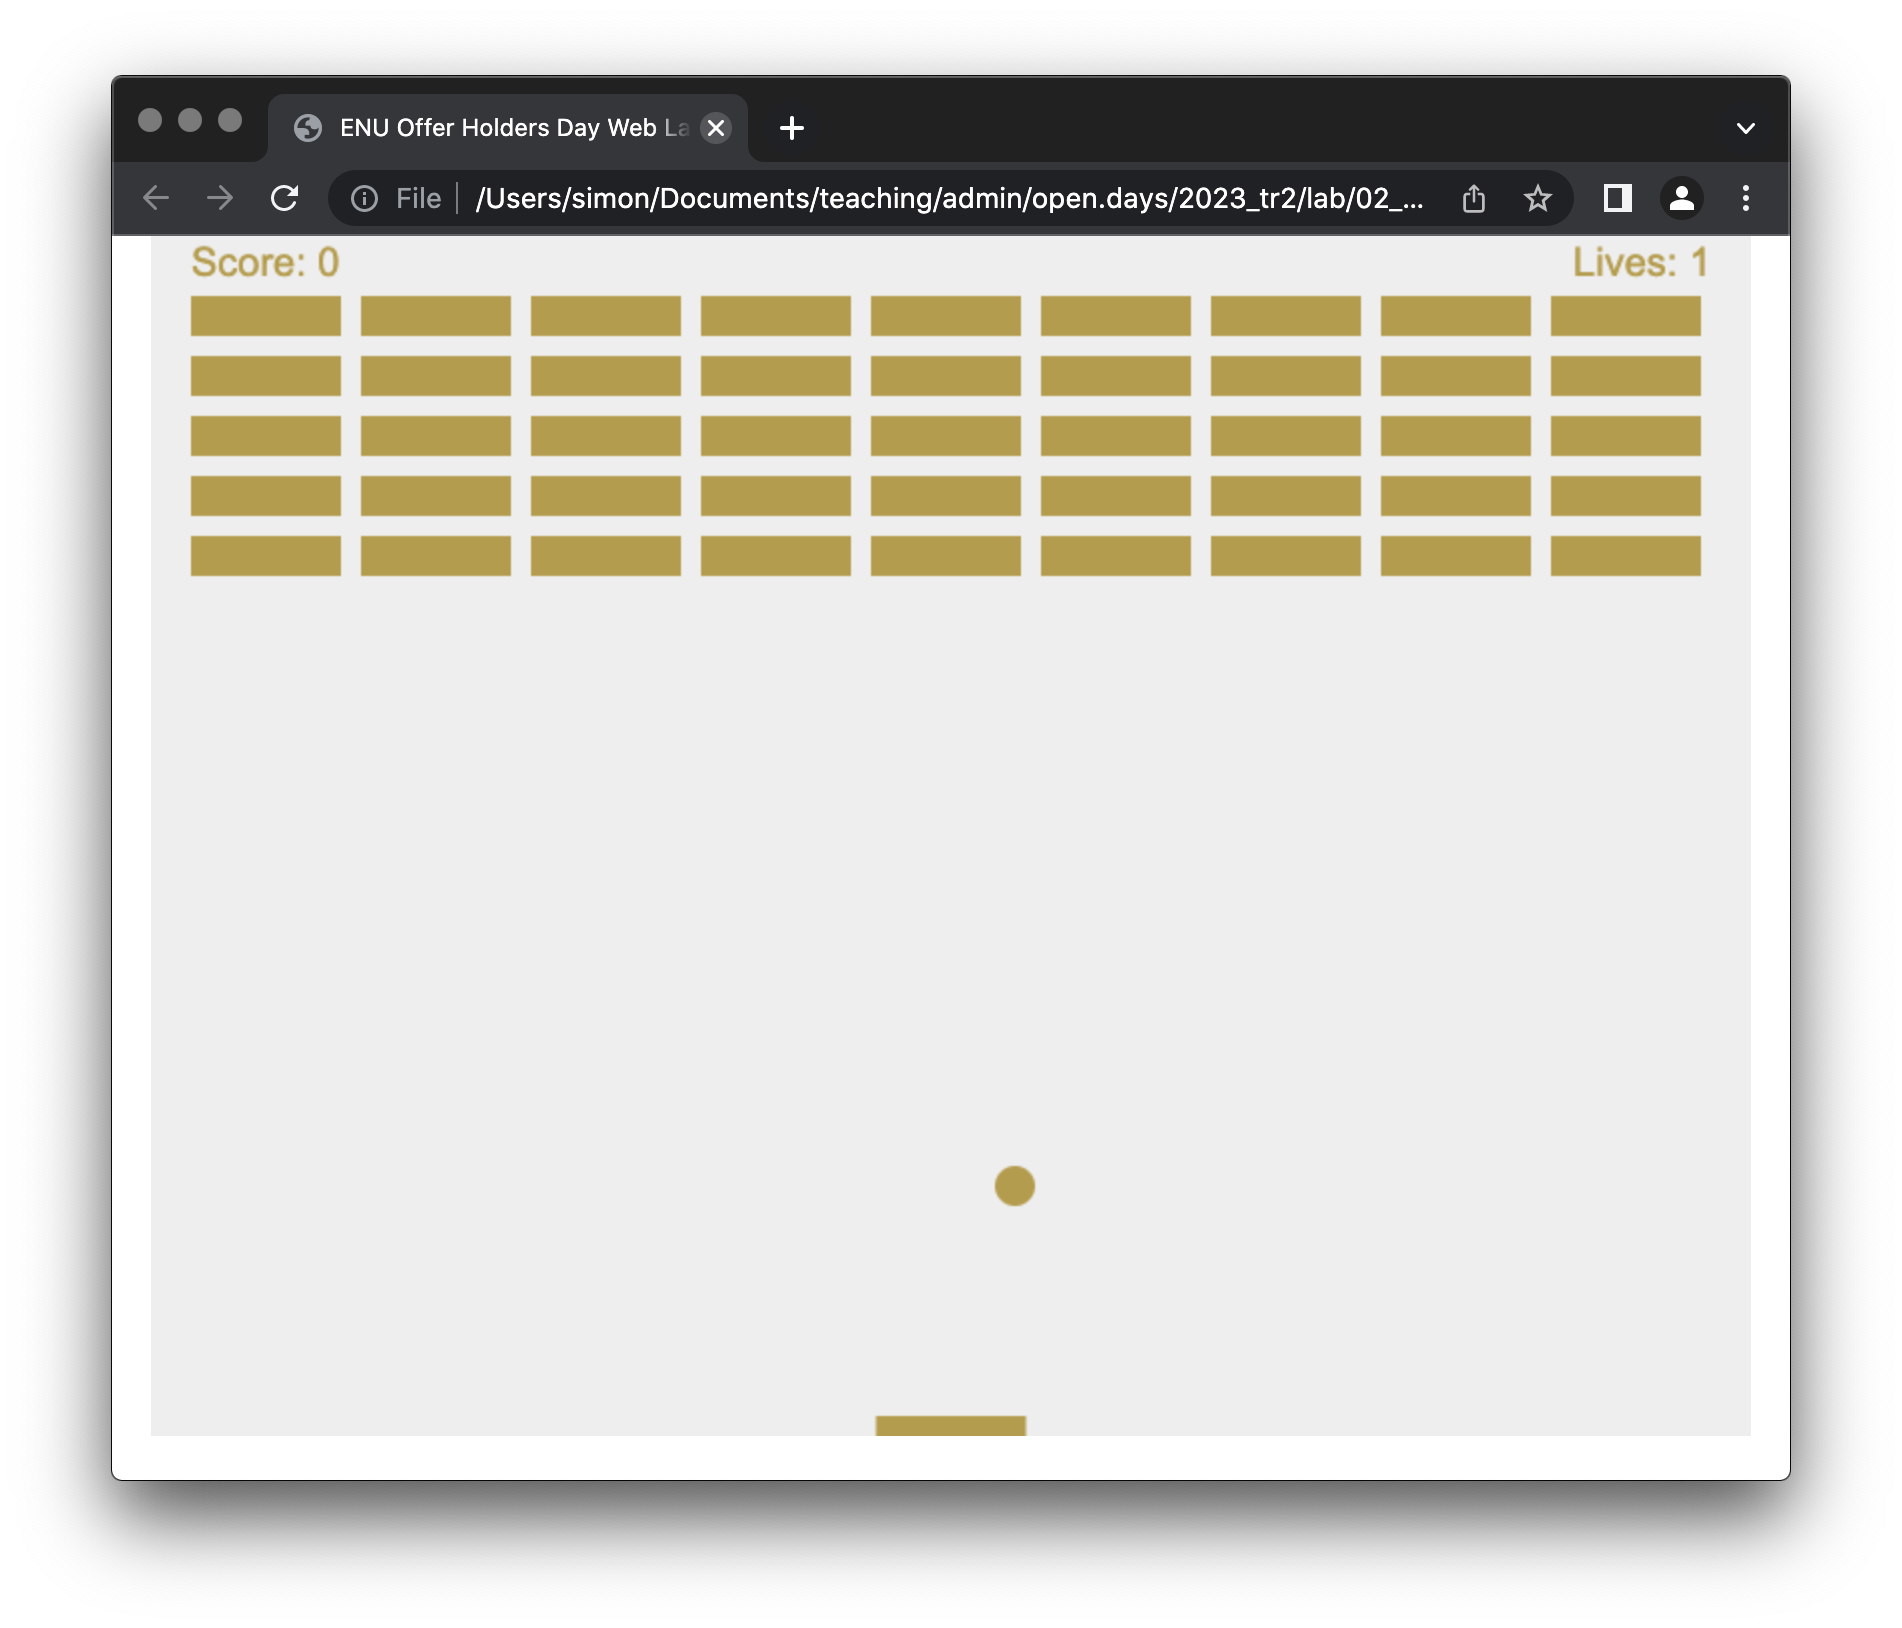
\includegraphics[width=0.8\textwidth]{images/02_drawing+d_draw_text.png}
\caption{Drawing the text.}
\label{fig:02_drawing+d_draw_text}
\end{figure}



\subsection{Gameloop}

\paragraph{} The game loop is something that happens in all games. It encapsulates the idea that we set up our game world, interact with the game world, update the game world as a result of the interaction, check for an end state, and then loop around to checking the interaction again. This loop continues until the game is finished.

\begin{lstlisting}
<!DOCTYPE html>
<html>
<head>
    <meta charset="utf-8" />
    <title>ENU Offer Holders Day Web Lab</title>
    <style>
        * { 
            padding: 0; 
            margin: 0; 
        } 
        canvas { 
            padding: 0; 
            margin: auto; 
            background: #eee; 
            display: block; 
        }
   </style>
</head>
<body>
    <canvas id="game_canvas" width="800" height="600"></canvas>

    <script>
        var canvas = document.getElementById("game_canvas");
        var ctx = canvas.getContext("2d");
        var ball_radius = 10;
        var x = canvas.width-Math.floor(Math.random()*750);
        var y = canvas.height-(Math.floor(Math.random()*200)+50);
        var paddle_height = 10;
        var paddle_width = 75;
        var paddle_position = (canvas.width-paddle_width)/2;
        var block_column_count = 9;
        var block_row_count = 5;
        var block_height = 20;
        var block_width = 75;
        var gutter = 10;
        var padding = 30;
        var top_margin = 20;
        var inside_margin = 20;
        var velocity = 4;
        var dx = Math.random() < 0.5 ? velocity : -velocity;
        var dy = -velocity;
        var score = 0;
        var lives = 1;
        var blocks = [];
        var colour = get_random_colour();

        function get_random_colour() {
            return '#'+Math.floor(Math.random()*16777215).toString(16);
        }

        function build_wall() {
            for(var c=0; c<block_row_count; c++) {
                blocks[c] = [];
                for(var r=0; r<block_column_count; r++) {
                    blocks[c][r] = { x: 0, y: 0, status: 1 };
                }
            }
        }
        build_wall();

        function draw_ball() {
            ctx.beginPath();
            ctx.arc(x, y, ball_radius, 0, Math.PI*2);
            ctx.fillStyle = colour;
            ctx.fill();
            ctx.closePath();
        }

        function draw_paddle() {
            ctx.beginPath();
            ctx.rect(paddle_position, canvas.height-paddle_height, paddle_width, paddle_height);
            ctx.fillStyle = colour;
            ctx.fill();
            ctx.closePath();
        }

        function draw_blocks() {
            for(var c=0; c<block_row_count; c++) {
                for(var r=0; r<block_column_count; r++) {
                    if(blocks[c][r].status == 1) {
                        var blockX = (r*(block_width+gutter))+inside_margin;
                        var blockY = (c*(block_height+gutter))+padding;
                        blocks[c][r].x = blockX;
                        blocks[c][r].y = blockY;
                        ctx.beginPath();
                        ctx.rect(blockX, blockY, block_width, block_height);
                        ctx.fillStyle = colour;
                        ctx.fill();
                        ctx.closePath();
                    }
                }
            }
        }

        function draw_score_text() {
            ctx.font = "20px Arial";
            ctx.fillStyle = colour;
            txt  = "Score: "+score;
            ctx.fillText(txt, inside_margin, top_margin);
        }

        function draw_lives_text() {
            ctx.font = "20px Arial";
            ctx.fillStyle = colour;
            txt = "Lives: "+lives;
            ctx.fillText(txt, canvas.width-(ctx.measureText(txt).width + inside_margin), top_margin );
        }

        function game_loop() {
            ctx.clearRect(0, 0, canvas.width, canvas.height);
            draw_blocks();
            draw_ball();
            draw_paddle();
            draw_score_text();
            draw_lives_text();
            requestAnimationFrame(game_loop);
        }
        
        game_loop();
    </script>
</body>
</html>
\end{lstlisting}

\paragraph{} To turn our collection of drawing functions into a rudimentary game we only need to do one thing:

\begin{description}
\item[Lines 109--117] This is where we get our code to loop over itself, to draw the world, then move the ball, then redraw the world, \emph{ad infinitum}. We've basically take all of our earierl calls to our draw functions and wrappe them in a function called game\_loop(). In line 116 we call requestAnimationFrame(), a canvas function that causes our code in the game\_loop function to be repeatedly called. At each cycle through the game loop we get a new frame of the game drawn to the screen. All of these frames give the illusion of continuous animation. This is the basis of all arcade style game interactions, basically draw the world to the screen sufficiently frequently, incorporating any updates or changes, so as to give the illusion of continuous change.
\item[Line 119] Here we call the game loop function. Once we've called it the first time it will call itself again, from within itself which will cause the drawing and move functions to be called over and over again.
\end{description}

\paragraph{} We still have a few things to do get our game complete but first, open the breakout.html file in Chrome and see how it looks. Your page should now look something like this (which isn't hugely different from how it looked before because the gameloop doesn't add anything visually impactful to out game. For this reason, we'll not bother with any more screenshots now until the final game):

\begin{figure}[H]
\centering
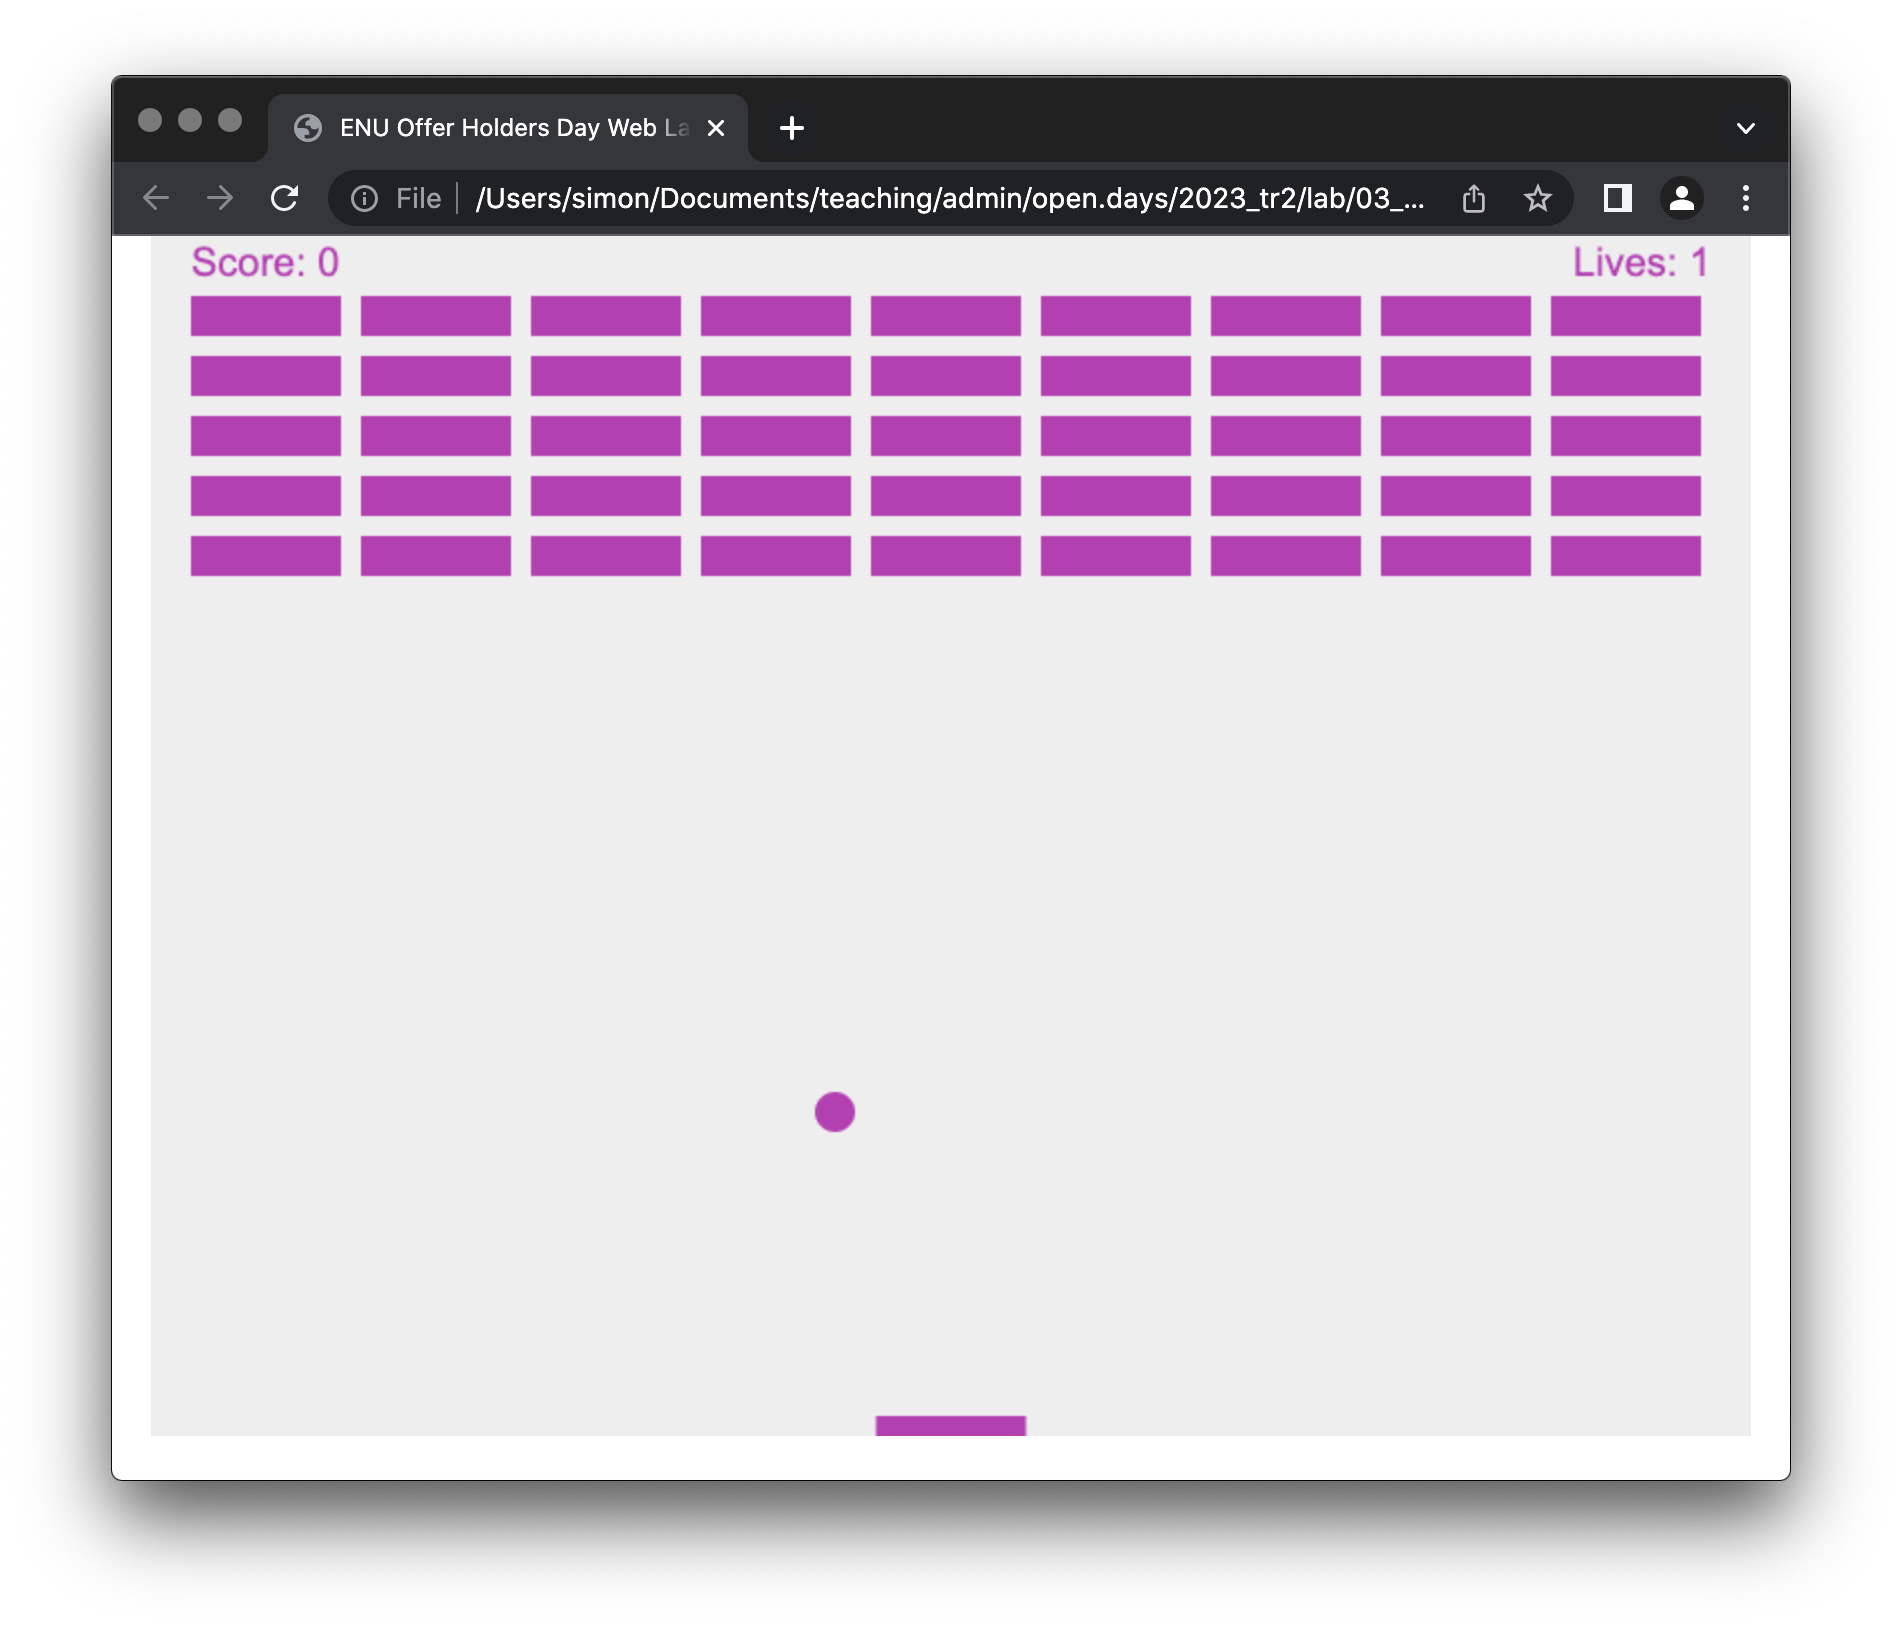
\includegraphics[width=0.8\textwidth]{images/03_gameloop+gameloop.png}
\caption{With a game loop to draw new frames as the ``game world'' changes.}
\label{fig:03_gameloop+gameloop}
\end{figure}


\subsection{Interaction}

\paragraph{} There are few forms of interaction within a game. One is the interaction of game objects between themselves, e.g. the ball interacting with the walls and bouncing off them. The other interaction is between the user and the game. We'll look at the ball's interaction first and then handle the user.

\begin{lstlisting}
<!DOCTYPE html>
<html>
<head>
    <meta charset="utf-8" />
    <title>ENU Offer Holders Day Web Lab</title>
    <style>
        * { 
            padding: 0; 
            margin: 0; 
        } 
        canvas { 
            padding: 0; 
            margin: auto; 
            background: #eee; 
            display: block; 
        }
   </style>
</head>
<body>
    <canvas id="game_canvas" width="800" height="600"></canvas>

    <script>
        var canvas = document.getElementById("game_canvas");
        var ctx = canvas.getContext("2d");
        var ball_radius = 10;
        var x = canvas.width-Math.floor(Math.random()*750);
        var y = canvas.height-(Math.floor(Math.random()*200)+50);
        var paddle_height = 10;
        var paddle_width = 75;
        var paddle_position = (canvas.width-paddle_width)/2;
        var block_column_count = 9;
        var block_row_count = 5;
        var block_height = 20;
        var block_width = 75;
        var gutter = 10;
        var padding = 30;
        var top_margin = 20;
        var inside_margin = 20;
        var velocity = 4;
        var dx = Math.random() < 0.5 ? velocity : -velocity;
        var dy = -velocity;
        var score = 0;
        var lives = 1;
        var blocks = [];
        var colour = get_random_colour();

        function get_random_colour() {
            return '#'+Math.floor(Math.random()*16777215).toString(16);
        }

        function build_wall() {
            for(var c=0; c<block_row_count; c++) {
                blocks[c] = [];
                for(var r=0; r<block_column_count; r++) {
                    blocks[c][r] = { x: 0, y: 0, status: 1 };
                }
            }
        }
        build_wall();

        function move() {
            if(x + dx > canvas.width-ball_radius || x + dx < ball_radius) {
                dx = -dx;
            }
            if(y + dy <= ball_radius) {
                dy = -dy;
            }
            else if(y + dy > canvas.height-ball_radius) {
                if(x > paddle_position && x < paddle_position + paddle_width) {
                    dy = -dy;
                }
                else {
                    lives--;
                    if(!lives) {
                        alert("GAME OVER");
                        document.location.reload();
                    }
                    else {
                        x = canvas.width-Math.floor(Math.random()*750+1);
                        y = canvas.height-Math.floor(Math.random()*250+1);                    
                        dx = Math.random() < 0.5 ? velocity : -velocity;
                        dy = -velocity;
                        paddle_position = (canvas.width-paddle_width)/2;
                    }
                }
            }
            x += dx;
            y += dy;
        }

        function draw_ball() {
            ctx.beginPath();
            ctx.arc(x, y, ball_radius, 0, Math.PI*2);
            ctx.fillStyle = colour;
            ctx.fill();
            ctx.closePath();
        }

        function draw_paddle() {
            ctx.beginPath();
            ctx.rect(paddle_position, canvas.height-paddle_height, paddle_width, paddle_height);
            ctx.fillStyle = colour;
            ctx.fill();
            ctx.closePath();
        }

        function draw_blocks() {
            for(var c=0; c<block_row_count; c++) {
                for(var r=0; r<block_column_count; r++) {
                    if(blocks[c][r].status == 1) {
                        var blockX = (r*(block_width+gutter))+inside_margin;
                        var blockY = (c*(block_height+gutter))+padding;
                        blocks[c][r].x = blockX;
                        blocks[c][r].y = blockY;
                        ctx.beginPath();
                        ctx.rect(blockX, blockY, block_width, block_height);
                        ctx.fillStyle = colour;
                        ctx.fill();
                        ctx.closePath();
                    }
                }
            }
        }

        function draw_score_text() {
            ctx.font = "20px Arial";
            ctx.fillStyle = colour;
            txt  = "Score: "+score;
            ctx.fillText(txt, inside_margin, top_margin);
        }

        function draw_lives_text() {
            ctx.font = "20px Arial";
            ctx.fillStyle = colour;
            txt = "Lives: "+lives;
            ctx.fillText(txt, canvas.width-(ctx.measureText(txt).width + inside_margin), top_margin );
        }

        
        draw_blocks();
        draw_ball();
        draw_paddle();
        draw_score_text();
        draw_lives_text();

        function game_loop() {
            ctx.clearRect(0, 0, canvas.width, canvas.height);
            draw_blocks();
            draw_ball();
            draw_paddle();
            draw_score_text();
            draw_lives_text();
            move();
            requestAnimationFrame(game_loop);
        }
        
        game_loop();
    </script>
</body>
</html>
\end{lstlisting}

\paragraph{} 

\begin{description}
\item[Lines 61--89] This is the move() function. It will move the ball each time we want to redraw the screen. In lines 62--64 it checks the location of the ball in relation to the left and right edges of the canvas and alters the ball location as a result if the ball hasn't gone out of bounds. In lines 65--67 we do a similar thing for the top edge of the canvas. In both cases, if the ball has reached the edge then we need to reflect the ball back in the opposite direction as if it were bouncing off the side or top walls. Line 68 checks whether the ball has reached the lower bound of the canvas. Lines 69--71 check whether the ball is colliding with the paddle and bounce it off if so. If the ball has reached the lower bound of the canvas but not hit the paddle then the player loses a life. This is handled by lines 72--86. Lines 73--77 deal with the case where the paddle misses the ball and the player has no more lives. In which case we use the alert() function to tell the user that the game is over. When the alert is cleared by clicking the OK button then the page is reloaded to give us a fresh game. Lines 78--84 however handle the case where the player lost a life but still has remaining lives, in which case we restart by ``serving'' the ball towards the wall again. Finally lines 87--88 handle the actual movement of the ball by updating the x and y coordinates once all those previous checks and updates have been completed. This is one of our more complex functions and has a number of moving parts but is integral to the game as we have to check each different context in which the ball can interact with the game's ``world''.\end{description}


\paragraph{} Now let's look at the user interaction. which is basically moving the paddle around to try to bounce the ball back towards the wall.


\begin{lstlisting}
<!DOCTYPE html>
<html>
<head>
    <meta charset="utf-8" />
    <title>ENU Offer Holders Day Web Lab</title>
    <style>
        * { 
            padding: 0; 
            margin: 0; 
        } 
        canvas { 
            padding: 0; 
            margin: auto; 
            background: #eee; 
            display: block; 
        }
   </style>
</head>
<body>
    <canvas id="game_canvas" width="800" height="600"></canvas>

    <script>
        var canvas = document.getElementById("game_canvas");
        var ctx = canvas.getContext("2d");
        var ball_radius = 10;
        var x = canvas.width-Math.floor(Math.random()*750);
        var y = canvas.height-(Math.floor(Math.random()*200)+50);
        var paddle_height = 10;
        var paddle_width = 75;
        var paddle_position = (canvas.width-paddle_width)/2;
        var block_column_count = 9;
        var block_row_count = 5;
        var block_height = 20;
        var block_width = 75;
        var gutter = 10;
        var padding = 30;
        var top_margin = 20;
        var inside_margin = 20;
        var velocity = 4;
        var dx = Math.random() < 0.5 ? velocity : -velocity;
        var dy = -velocity;
        var score = 0;
        var lives = 1;
        var blocks = [];
        var colour = get_random_colour();

        document.addEventListener("mousemove", mouse_move_handler, false);

        function get_random_colour() {
            return '#'+Math.floor(Math.random()*16777215).toString(16);
        }

        function build_wall() {
            for(var c=0; c<block_row_count; c++) {
                blocks[c] = [];
                for(var r=0; r<block_column_count; r++) {
                    blocks[c][r] = { x: 0, y: 0, status: 1 };
                }
            }
        }
        build_wall();
        
        function mouse_move_handler(e) {
            var relative_x = e.clientX - canvas.offsetLeft;
            if(relative_x > 0 && relative_x < canvas.width) {
                paddle_position = relative_x - paddle_width/2;
            }
        }

        function move() {
            if(x + dx > canvas.width-ball_radius || x + dx < ball_radius) {
                dx = -dx;
            }
            if(y + dy <= ball_radius) {
                dy = -dy;
            }
            else if(y + dy > canvas.height-ball_radius) {
                if(x > paddle_position && x < paddle_position + paddle_width) {
                    dy = -dy;
                }
                else {
                    lives--;
                    if(!lives) {
                        alert("GAME OVER");
                        document.location.reload();
                    }
                    else {
                        x = canvas.width-Math.floor(Math.random()*750+1);
                        y = canvas.height-Math.floor(Math.random()*250+1);                    
                        dx = Math.random() < 0.5 ? velocity : -velocity;
                        dy = -velocity;
                        paddle_position = (canvas.width-paddle_width)/2;
                    }
                }
            }
            x += dx;
            y += dy;
        }

        function draw_ball() {
            ctx.beginPath();
            ctx.arc(x, y, ball_radius, 0, Math.PI*2);
            ctx.fillStyle = colour;
            ctx.fill();
            ctx.closePath();
        }

        function draw_paddle() {
            ctx.beginPath();
            ctx.rect(paddle_position, canvas.height-paddle_height, paddle_width, paddle_height);
            ctx.fillStyle = colour;
            ctx.fill();
            ctx.closePath();
        }

        function draw_blocks() {
            for(var c=0; c<block_row_count; c++) {
                for(var r=0; r<block_column_count; r++) {
                    if(blocks[c][r].status == 1) {
                        var blockX = (r*(block_width+gutter))+inside_margin;
                        var blockY = (c*(block_height+gutter))+padding;
                        blocks[c][r].x = blockX;
                        blocks[c][r].y = blockY;
                        ctx.beginPath();
                        ctx.rect(blockX, blockY, block_width, block_height);
                        ctx.fillStyle = colour;
                        ctx.fill();
                        ctx.closePath();
                    }
                }
            }
        }

        function draw_score_text() {
            ctx.font = "20px Arial";
            ctx.fillStyle = colour;
            txt  = "Score: "+score;
            ctx.fillText(txt, inside_margin, top_margin);
        }

        function draw_lives_text() {
            ctx.font = "20px Arial";
            ctx.fillStyle = colour;
            txt = "Lives: "+lives;
            ctx.fillText(txt, canvas.width-(ctx.measureText(txt).width + inside_margin), top_margin );
        }
        
        function game_loop() {
            ctx.clearRect(0, 0, canvas.width, canvas.height);
            draw_blocks();
            draw_ball();
            draw_paddle();
            draw_score_text();
            draw_lives_text();
            move();
            requestAnimationFrame(game_loop);
        }
        
        game_loop();
    </script>
</body>
</html>
\end{lstlisting}

\paragraph{} 

\begin{description}
\item[Line 47] Here we add an ``event handler'' to our HTML document. User interactions are events in which something has happened as a result of the user performing some action. In this case, our event handler is designed to fire off events when the user moves the mouse. When a mouse move event is detected then the handler automatically calls our mouse\_move\_handler() function which we'll look at next.
\item[Lines 63--68] This is our mouse\_move\_handler() function which is passed some variables when it is called. These variables store coordinates associated with the mouse move and we can use those to update the position of the paddle. First, line 64 we convert the incoming coordinates which refer to the browser window into coordinates associated with our canvas. We then check that the mouse coordinates are within the bounds of the canvas (line 65) and if they are, we update the position of the paddle to reflect whether the mouse has moved left or right. In essence, we track the horizontal movement of the mouse pointer and move the paddle left or right as a result.
\end{description}

\paragraph{} Our mouse moving the paddle, in combination with the move() function from earlier means that we can now interact with our game. So we can bounce the ball off the paddle, back towards the wall. Of course we haven't yet added code to handle interactions between the ball and the blocks that make up the wall yet, but that'll be our next, and final, task.

\subsection{Collisions}
\label{section:collisions}

\paragraph{} In this final sub-section, we'll add the final function needed for our complete game. So let's get on with it. As before, here's the full code listing (which is actually the full and final code listing for the lab):

\begin{lstlisting}
<!DOCTYPE html>
<html>
<head>
    <meta charset="utf-8" />
    <title>ENU Offer Holders Day Web Lab</title>
    <style>
        * { 
            padding: 0; 
            margin: 0; 
        } 
        canvas { 
            padding: 0; 
            margin: auto; 
            background: #eee; 
            display: block; 
        }
   </style>
</head>
<body>
    <canvas id="game_canvas" width="800" height="600"></canvas>

    <script>
        var canvas = document.getElementById("game_canvas");
        var ctx = canvas.getContext("2d");
        var ball_radius = 10;
        var x = canvas.width-Math.floor(Math.random()*750);
        var y = canvas.height-(Math.floor(Math.random()*200)+50);
        var paddle_height = 10;
        var paddle_width = 75;
        var paddle_position = (canvas.width-paddle_width)/2;
        var block_column_count = 9;
        var block_row_count = 5;
        var block_height = 20;
        var block_width = 75;
        var gutter = 10;
        var padding = 30;
        var top_margin = 20;
        var inside_margin = 20;
        var velocity = 4;
        var dx = Math.random() < 0.5 ? velocity : -velocity;
        var dy = -velocity;
        var score = 0;
        var lives = 1;
        var blocks = [];
        var colour = get_random_colour();

        document.addEventListener("mousemove", mouse_move_handler, false);

        function get_random_colour() {
            return '#'+Math.floor(Math.random()*16777215).toString(16);
        }

        function build_wall() {
            for(var c=0; c<block_row_count; c++) {
                blocks[c] = [];
                for(var r=0; r<block_column_count; r++) {
                    blocks[c][r] = { x: 0, y: 0, status: 1 };
                }
            }
        }
        build_wall();
        
        function mouse_move_handler(e) {
            var relative_x = e.clientX - canvas.offsetLeft;
            if(relative_x > 0 && relative_x < canvas.width) {
                paddle_position = relative_x - paddle_width/2;
            }
        }

        function collision_detection() {
            for(var c=0; c<block_row_count; c++) {
                for(var r=0; r<block_column_count; r++) {
                    var block = blocks[c][r];
                    if(block.status == 1) {
                        if(x > block.x && x < block.x+block_width && y > block.y && y < block.y+block_height) {
                            dy = -dy;
                            block.status = 0;
                            score++;
                            if(score == block_column_count*block_row_count) {
                                alert("WINNER! WINNER!");
                                document.location.reload();
                            }
                        }
                    }
                }
            }
        }

        function move() {
            if(x + dx > canvas.width-ball_radius || x + dx < ball_radius) {
                dx = -dx;
            }
            if(y + dy <= ball_radius) {
                dy = -dy;
            }
            else if(y + dy > canvas.height-ball_radius) {
                if(x > paddle_position && x < paddle_position + paddle_width) {
                    dy = -dy;
                }
                else {
                    lives--;
                    if(!lives) {
                        alert("GAME OVER");
                        document.location.reload();
                    }
                    else {
                        x = canvas.width-Math.floor(Math.random()*750+1);
                        y = canvas.height-Math.floor(Math.random()*250+1);                    
                        dx = Math.random() < 0.5 ? velocity : -velocity;
                        dy = -velocity;
                        paddle_position = (canvas.width-paddle_width)/2;
                    }
                }
            }
            x += dx;
            y += dy;
        }

        function draw_ball() {
            ctx.beginPath();
            ctx.arc(x, y, ball_radius, 0, Math.PI*2);
            ctx.fillStyle = colour;
            ctx.fill();
            ctx.closePath();
        }

        function draw_paddle() {
            ctx.beginPath();
            ctx.rect(paddle_position, canvas.height-paddle_height, paddle_width, paddle_height);
            ctx.fillStyle = colour;
            ctx.fill();
            ctx.closePath();
        }

        function draw_blocks() {
            for(var c=0; c<block_row_count; c++) {
                for(var r=0; r<block_column_count; r++) {
                    if(blocks[c][r].status == 1) {
                        var blockX = (r*(block_width+gutter))+inside_margin;
                        var blockY = (c*(block_height+gutter))+padding;
                        blocks[c][r].x = blockX;
                        blocks[c][r].y = blockY;
                        ctx.beginPath();
                        ctx.rect(blockX, blockY, block_width, block_height);
                        ctx.fillStyle = colour;
                        ctx.fill();
                        ctx.closePath();
                    }
                }
            }
        }

        function draw_score_text() {
            ctx.font = "20px Arial";
            ctx.fillStyle = colour;
            txt  = "Score: "+score;
            ctx.fillText(txt, inside_margin, top_margin);
        }

        function draw_lives_text() {
            ctx.font = "20px Arial";
            ctx.fillStyle = colour;
            txt = "Lives: "+lives;
            ctx.fillText(txt, canvas.width-(ctx.measureText(txt).width + inside_margin), top_margin );
        }

        function game_loop() {
            ctx.clearRect(0, 0, canvas.width, canvas.height);
            draw_blocks();
            draw_ball();
            draw_paddle();
            draw_score_text();
            draw_lives_text();
            collision_detection();
            move();
            requestAnimationFrame(game_loop);
        }
        
        game_loop();
    </script>
</body>
</html>
\end{lstlisting}

\paragraph{} The main thing to note this time is the addition of the collision\_detection() function

\begin{description}
\item[Lines 70--87] This is our collision\_detection() function. All we're doing in this function is looping through our blocks array, using a pair of nested \emph{for} loops to visit every block in the wall. For each block we check whether it has already been hit by the ball and if so then we ignore it. If a block hasn't yet been hit then we check to see whether the ball is going to hit it using the coordinates of the ball and the coordinates of the block. If the ball will hit the block then we change the status of the block so that it is removed from the wall in the next iteration of the game loop, then we reverse the direction of the ball as though it bounced from the block when it destroyed it. Finally we do a quick check to determine if the block that was hit was the final block and if it was then the game is won because all of the blocks have been destroyed. At this point, as for losing the game in the move() function, we use an alert to tell the player that they won and then reload the document to start a new game once the player clears the alert.
\item[Lines 174] Finally, we call collision\_detection() from within the game loop.
\end{description}

\paragraph{} If you open your breakout.html file in Chrome it should look something similar to this:

\begin{figure}[H]
\centering
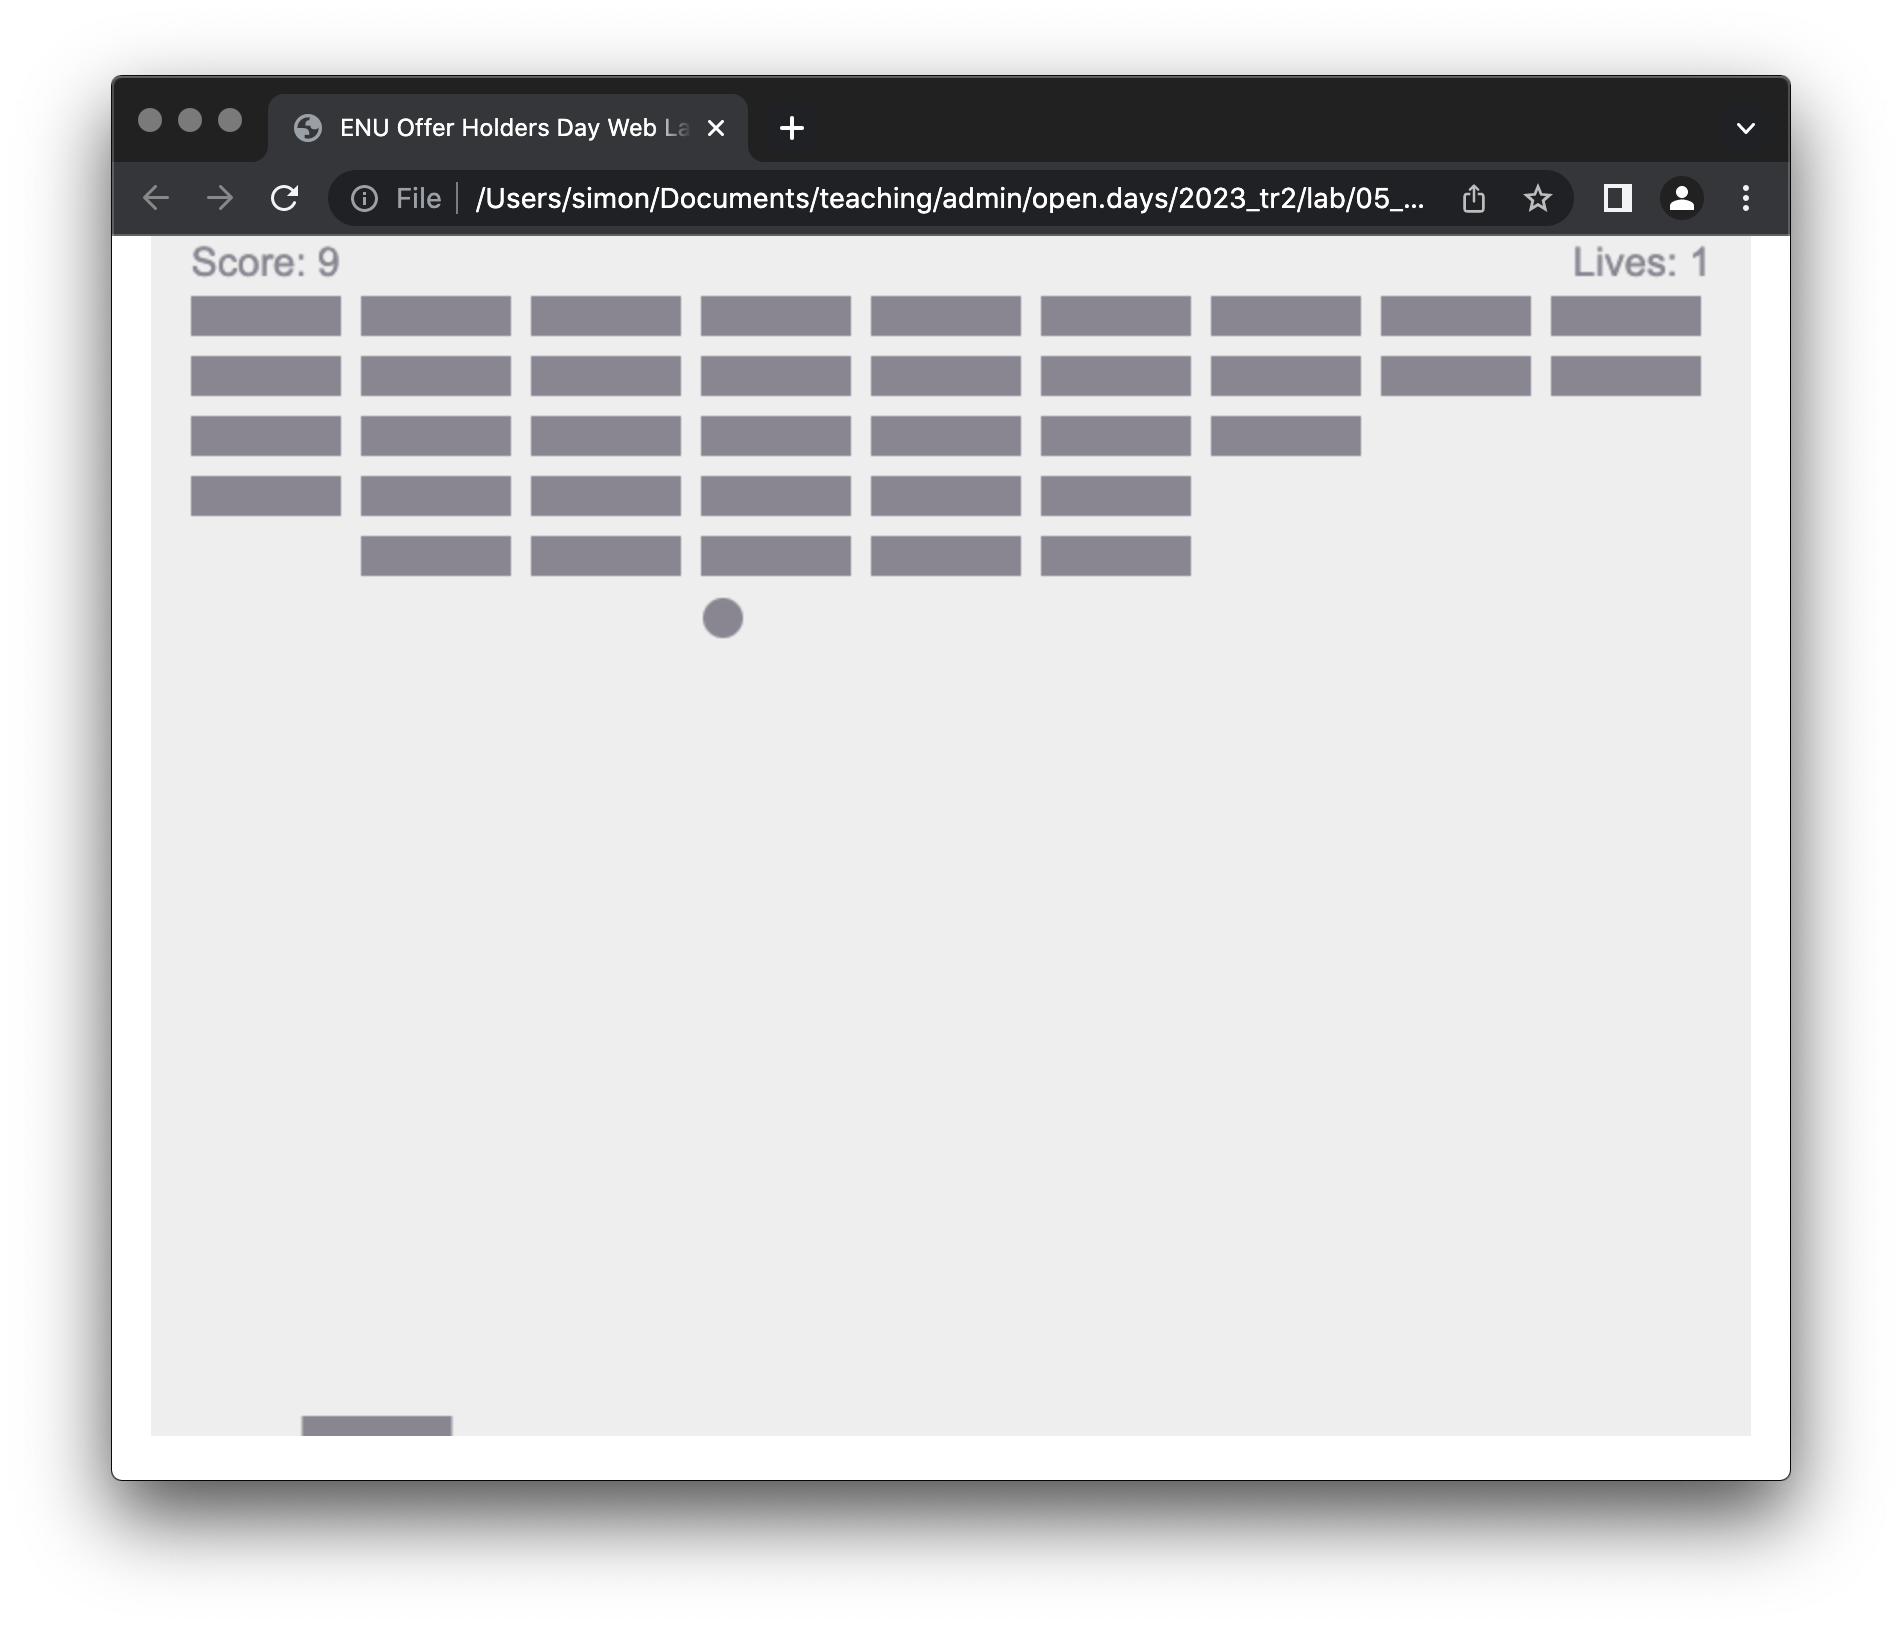
\includegraphics[width=0.8\textwidth]{images/05_collisions+collisions.png}
\caption{The final game, with collisions removing blocks from the wall.}
\label{fig:05_collisions+collisions}
\end{figure}


\paragraph{} And that's it folks. You now have a simple, playable, browser-hosted Javascript game in fewer than 200 lines of code. Obviously there's way more to learn about coding in HTML, CSS, \& Javascript than we've covered here but I'm hoping it's whetted your apetite for more.

\subsection{Challenge}
\label{section:challenges}
\paragraph{} I'm interested to see where you can take this in the time between today and when you arrive for your first trimester. Here are some ideas:

\begin{itemize}
\item Work out how to alter the number of lives available.
\item Work out how to alter the size of the ball.
\item Work out how to alter the size of the paddle.
\item Work out how to alter the speed at which the ball moves.
\item What would you need to do to have more than one ``level''? What would other levels include? Perhaps a faster ball? Or a different pattern of blocks? What if the blocks needed more than one strike to destroy them?
\item What about special blocks that give power ups? Perhaps multiple balls for a short duration? Or a superball that blasts through the blocks until it rebounds off a wall? Or a larger paddle for a given duration?
\item Visually you could alter things as well. What about colouring the blocks and other aspects of the game in different ways? If you are just using random colours this could be visually cacophonous so consider how you might ensure that the colour palette is cohesive.
\item The physics model that we have for things like the ball rebounding is very rudimentary. It might be nice if, for example, the angel of rebound of the ball changed when hit by a rapidly moving paddle instead of a static paddle, a bit like how a tennis ball responds differently depending upon how it is struck.
\item Also consider things like sound effects. Even a single sound that plays at certain events such as losing a ball, destroying a block, or rebounding from the wall can greatly change the users experience.
\item The classic breakout game isn't too far away from other classic games like Space Invaders. If the blocks could move, and perhaps fired back, and the paddle fired multiple balls one after the other, which didn't rebound, then you'd have most of a space invaders game. Perhaps some of our breakout code would work to achieve that?
\end{itemize}

\paragraph{} Feel free to contact me to let me know how you get on and what you manage to achieve...

%\backmatter

\bibliographystyle{plain}

\bibliography{workbook}

\end{document}

%\begin{framed}
%HELLO
%\end{framed}


